\documentclass{amsart}
\usepackage{amsmath,amssymb,latexsym,color}
\usepackage[bookmarks=true,colorlinks=true, linkcolor=blue, citecolor=cyan]{hyperref}
\usepackage{tikz}
\usepackage{pgflibraryarrows}
\usepackage{pgflibrarysnakes}
\usetikzlibrary{fit}
\usepackage[margin=1in]{geometry}
\usepackage{extarrows}
\input xy
\xyoption{all}

\newtheorem{theorem}{Theorem}[section]
\newtheorem{claim}[theorem]{Claim}
\newtheorem{corollary}[theorem]{Corollary}
\newtheorem{definition}[theorem]{Definition}
\newtheorem{lemma}[theorem]{Lemma}
\newtheorem{question}[theorem]{Question}
\newtheorem{proposition}[theorem]{Proposition}
\newtheorem{remark}[theorem]{Remark}

\newcommand{\bfe}{\mathbf{e}}
\newcommand{\bff}{\mathbf{f}}
\newcommand{\bfg}{\mathbf{g}}
\newcommand{\bfi}{\mathbf{i}}
\newcommand{\bfh}{\mathbf{h}}
\newcommand{\tbfe}{{\tilde\bfe}}
\newcommand{\tbff}{{\tilde\bff}}
\newcommand{\tbfg}{{\tilde\bfg}}
\newcommand{\tbfh}{{\tilde\bfh}}
\newcommand{\C}{\mathbb{C}}
\newcommand{\cC}{\mathcal{C}}
\newcommand{\cG}{\mathcal{G}}
\newcommand{\cP}{\mathcal{P}}
\newcommand{\ui}{\underline i}
\newcommand{\uj}{\underline j}
\newcommand\udim{{\underline{\dim}\, }}
\newcommand{\pt}{\mathrm{pt}}
\newcommand{\Rep}{\mathrm{Rep}}
\newcommand{\rep}{\operatorname{rep}}
\newcommand{\Gr}{\mathrm{Gr}}
\renewcommand{\AA}{\mathbb{A}}
\newcommand{\CC}{\mathbb{C}}
\newcommand{\kk}{\Bbbk}
\newcommand{\ZZ}{\mathbb{Z}}
\newcommand{\Ext}{\operatorname{Ext}}
\newcommand{\Hom}{\operatorname{Hom}}
\newcommand{\im}{\operatorname{im}}
\newcommand{\codim}{\operatorname{codim}}
\newcommand{\into}{\hookrightarrow}
\newcommand{\onto}{\to\!\!\!\!\!\to}
\newcommand{\ses}[3]{0\rightarrow #1\rightarrow #2\rightarrow#3\rightarrow 0}
\newcommand{\Sc}[2]{\langle #1,#2\rangle}
\newcommand{\spn}{\operatorname{span}}
\setcounter{MaxMatrixCols}{20}
\title{Cell Decomposition of Rank 2 Quiver Grassmannians}

\author{Dylan Rupel}
\author{Thorsten Weist}

\begin{document}
\begin{abstract}
  We prove that all quiver Grassmannians for preprojective and preinjective representations of a generalized Kronecker quiver admit a cell decomposition.  
  We also provide a natural combinatorial labeling for these cells using compatible pairs in a maximal Dyck path. 
\end{abstract}
\maketitle

\section{Introduction}
A cluster algebra is a subalgebra of a rational function field where generators are defined by an explicit recursion \cite{fomin-zelevinsky}.
Although the generators of the cluster algebra are given as rational functions they actually turn out to be Laurent polynomials.
These Laurent polynomial expressions for the cluster variables have been studied extensively and ultimately can be described using the representation theory of quivers \cite{caldero-chapoton,caldero-keller}.


-something about categorification and quiver Grassmannians
-something about compatible pairs and combinatorial construction of cluster variables
-statement of our results
-something about torus actions and the universal cover
-something about cell decompositions of quiver Grassmannians
-acknowledgements?


%%%%%%%%%%%%%%%%%%%%%%%%%%%%%%%%%%%%%%%%%%%%%%
\section{Terminology and Preliminary results}
\subsection{Covering theory}\footnote{more and more precise definitions}
For an introduction to covering theory we refer to \cite{gab}. Let $Q$ be an acyclic quiver with vertices $Q_0$ and arrows $Q_1$ which we denote by $\alpha:i\to j$. We denote by $\Rep(Q)$ the category of $\C$-representations of $Q$. Moreover, let $A_Q\cong \ZZ^{Q_1}$ be the free abelian group and $W_{Q}$ be the free non-abelian group generated by $Q_1$.  
\begin{definition}
The universal abelian covering quiver $\hat Q$ of $Q$ is given by the vertices $\hat Q_0=Q_0\times A_{Q}$ and the arrow set $\hat Q_1=Q_1\times A_{Q}$ where $(\alpha,\chi):(i,\chi)\to (j,\chi+e_\alpha)$ for every $\alpha:i\to j$.

The universal covering quiver $\tilde Q$ of $Q$ is given by the vertices $\tilde Q_0=Q_0\times W_{Q}$ and the arrow set $\tilde Q_1=Q_1\times W_{Q}$ where $(\alpha,w):(i,w)\to (j,w\alpha)$ for every $\alpha:i\to j$.

We say that a representation $X\in \Rep(Q)$ can be lifted to $\hat Q$ (resp. $\tilde Q$) if there exists a representation $\hat X\in\Rep(\hat Q)$ (resp. $\tilde X\in\Rep(\tilde Q)$) such that $F_Q\hat X=X$ (resp. $G_Q \tilde X=X$) where $F_Q:\Rep(\hat Q)\to\Rep(Q)$ (resp. $G_Q:\Rep(\tilde Q)\to\Rep(Q)$) is the natural functor.
\end{definition}
Note that in our definition every covering quiver has infinitely many connected components. But every connected component is a covering in the sense of \cite{gab}. As indecomposable representations live on one component this makes no difference.
Note that we also have a natural functor $H_Q:\Rep(\tilde Q)\to \Rep(\hat Q)$.
Moreover, note that every connected component of the universal covering quiver of the universal abelian covering quiver is isomorphic to a connected component of the universal covering quiver of the original quiver. The functor $F_Q$ induces a map $F_Q:\ZZ^{\hat Q_1}\to \ZZ^{Q_1}$. We say that a dimension vector $\hat \bfe$ of $\hat Q$ is compatible with $\bfe$ if $F_Q(\hat\bfe)=\bfe$. The group $A_Q$ acts on $\hat Q$ via translation inducing an action on $\Rep(\hat Q)$ and on $\ZZ^{\hat Q_1}$. We say two representation (resp. dimension vectors) are equivalent in this case. The analogous observation can also be made for $\tilde Q$. If $M$ is a representation of $\hat Q$ (resp. $\tilde Q$), we denote the representation obtained by translation by $\chi\in A_Q$ (resp. $w\in W_Q$) by $M_\chi$ (resp. $M_w$).  


\begin{lemma}
  Every preprojective (resp. preinjective) representation of $Q$ can be lifted to  $\hat Q$ and $\tilde Q$.
\end{lemma}
\begin{proof}This statement is clear for the simple representations $S_q$, $q\in Q_0$. Now every preprojective representation $X$ can be obtained when applying a sequence of BGP-reflections \cite{bgp} to a simple representation $S_{q'}$ of a quiver $Q'$ whose underlying graph is the same as the one of $Q$. Applying BGP-reflections to a source $q$ of $Q$ corresponds to applying BGP-reflections to all vertices $(q,\chi)$ of $\hat Q$ (resp. $(q,w)$ of $\tilde Q$). This leads the claim. The statement for preinjective representations follows in the same way.
\end{proof}
As $F_Q$ and $G_Q$ are covering functors when restricting to one connected component, we obtain
\begin{theorem}\label{covering}
The functors $F_Q$ and $G_Q$ preserve indecomposability. Moreover, for all representations $\hat X,\hat Y \in\Rep(\hat Q)$, we have 
\[\Hom_Q(F_Q\hat X, F_Q\hat Y)\cong \bigoplus_{\chi\in A_Q}\Hom_{\tilde Q}(\hat X_\chi,\hat Y)\cong\bigoplus_{\chi\in A_Q}\Hom_{\tilde Q}(\hat X,\hat Y_\chi).\]
The analogous statement is true when replacing $\Hom$ by $\Ext$ and $\Rep(\hat Q)$ by $\Rep(\tilde Q)$ respectively.
\end{theorem}

Recall that every tuple of linear maps $(f_v:X_{s(v)}\to Y_{t(v)})_{v\in Q_1}$ defines a short exact sequence $\ses{Y}{Z}{X}$ with middle term defined by the vector spaces $Z_q=X_q\oplus Y_q$ for all $q\in Q_0$ and linear maps $Z_v=\begin{pmatrix}Y_v &f_v\\0&X_v\end{pmatrix}$ for all $v\in Q_1$. 
In general, considering the linear map  
\[d_{X,Y}:\bigoplus_{q\in Q_0}\Hom_k(X_q,Y_q)\to\bigoplus_{v\in Q_1}\Hom_k(X_{s(v)},Y_{t(v)}), (f_q)_{q\in Q_0}\mapsto(f_{t(v)}\circ X_{v}-Y_{s(v)}\circ f_{s(v)})_{v\in Q_1} \]
we have $\mathrm{ker}(d_{X,Y})=\Hom_Q(X,Y)$ and $\mathrm{coker}(d_{X,Y})=\Ext_Q(X,Y)$.



\subsection{Bialynicki-Birula decomposition}
The aim of Section \ref{torusaction} is to define a torus action on quiver Grassmannians which can be used to simplify the calculation of homological invariants in general. If the quiver Grassmannian is smooth, which is for instance the case for exceptional representations by \cite{cr}, it can also be used to stratify the quiver Grassmannians using the results of Bialynicki-Birula. More detailed, let $X$ be a smooth projective variety with a $\C^\ast$-action. For a connecting component of the fixed point set $C\subset X^{\C^\ast}$, we define its attracting set as
\[\mathrm{Att}(C):=\{y\in X\mid \lim_{t\to 0}t.y\in C\}\]

Then we have the following statement, \cite[Section 4]{bb}:
\begin{theorem}Let $\coprod_{i=1}^r C_i= X^{\C^\ast}$ be the decomposition into connected components. Then $\mathrm{Att}(C_i)$ is a locally closed smooth $\C^\ast$-invariant subvariety of $X$ where $C_i$ is a subvariety of $\mathrm{Att}(C_i)$. Moreover, we have $X=\coprod_{i=1}^r\mathrm{Att}(C_i)$ and
the natural map $\gamma_i:\mathrm{Att}(C_i)\to C_i$ is an affine vector bundle. 

In particular, we have $\chi(X)=\chi(X^{\C^\ast})$ for the Euler characteristic.
\end{theorem}
Let $\ses{M}{B}{N}$ be a short exact sequence of representations. This induces a map between quiver Grassmannians
\[\Psi_\tbfe:Gr_\tbfe(B)\to\bigsqcup_{\tbff+\tbfg=\tbfe}  Gr_\tbff(M)\times Gr_\tbfg(N),\,U\mapsto (U\cap M,(U+M)/M)\]
which is also called Caldero-Chapoton map.  By the results of \cite[Section 3]{cc} it follows that $\Psi^{-1}_\tbfe(A,V)=\mathbb{A}^{\dim\Hom(A,M/V)}$ for all pairs of subrepresentations $(A,V)$ for which the fibre is not empty.
Let $\cG_{\tbff,\tbfg}:=\Psi^{-1}_\tbfe(\Gr_\tbff(M)\times \Gr_\tbfg(N))$. Then we have
$$\Gr_\tbfe(B)=\bigsqcup_{\tbff+\tbfg=\tbfe} \cG_{\tbff,\tbfg}.$$
The map $\Psi_\tbfe$ restricts to morphisms of projective varieties
\[\Psi_\tbfe^{\tbff,\tbfg}:\cG_{\tbff,\tbfg}\to \Gr_\tbff(M)\times \Gr_\tbfg(N).\]

The following is proved in \cite[Section 3]{cefr}.
\begin{theorem}\label{vb}
If the fibre dimension of $\Psi_\tbfe^{\tbff,\tbfg}$ is constant over $\mathrm{Im}(\Psi_\tbfe^{\tbff,\tbfg})$, then it an affine bundle over the image. In particular, the existence of a cell decomposition of $\mathrm{Im}(\Psi_\tbfe^{\tbff,\tbfg})$ implies a cell decomposition of $\cG_{\tbff,\tbfg}$ in this case.
\end{theorem}
\begin{proof}\footnote{sketch, double-check}


As $X$ and $Y$ are projective, they are compact. As the fibres are affine spaces of constant dimension and as $X$ and $Y$ are smooth, the induced morphism on the tangent spaces is surjective for all points $x\in X$. This shows that $f$ is smooth of relative dimension $n$, see Hartshorne and thus a submersion?!



\end{proof}
\section{Torus Actions on Quiver Grassmannians}\label{torusaction}
\noindent 
Fix a vector space $X$ of dimension $n$ and let $d\leq n$. We first consider a natural torus action on usual Grassmannians coming along with any direct sum decomposition of the vector space $X$. Then we generalize the concept to quiver Grassmannians, but we will see that the torus fixed point set can be calculated in an analogous manner. Thus assume that $X=\bigoplus_{j=1}^l X_j$ is a direct sum decomposition of $X$. We choose a basis $\mathcal B=\{v_1,\ldots,v_n\}$ of $X$ which is compatible with this decomposition, i.e. there exist numbers $1\leq j_1\leq j_2\ldots\leq j_{l-1}\leq n$ such that
\[v_1,\ldots,v_{j_1}\in X_1,\,v_{j_1+1},\ldots,v_{j_2}\in X_2,\ldots,v_{j_{l-1}+1},\ldots,v_{n}\in X_l\]
Moreover, we choose a map $d:\{1,\ldots,n\}\to\mathbb{Z}$ such that $d(i)=d(i')$ if $v_i,v_{i'}\in X_{j}$ for some $j$. Then there exists a $\C^\ast$-action on $X$ when extending the definition $t.v_i:=t^{d(j)}v_i$ if $v_i\in X_j$ linearly to $X$. This naturally induces an action of $\C^\ast$ on the usual Grassmannians $\Gr_d(X)$. We can write every $U\in\Gr_d(X)$ uniquely in row-echelon form with respect to the basis $\mathcal B$, i.e. there exists a unique sequence $1\leq i_1\leq\ldots\leq i_d\leq n$ and a unique matrix representation of $U$ of the form
\[M(U):=\begin{pmatrix}\ast&\ldots &\ast &1&0 &\ldots&\ldots&\ldots&\ldots&\ldots&\ldots&\ldots&\ldots&\ldots&0\\\ast&\ldots &\ast&0&\ast&\ldots &\ast&1&0&\ldots&\ldots&\ldots&\ldots&\ldots&0\\\vdots &\ddots&\vdots&\vdots&\vdots &\ddots&\vdots&0&\ast&\ddots&\ddots&\ddots&\ddots&\ddots&\vdots\\\vdots &\ddots&\vdots&\vdots&\vdots &\ddots&\vdots&\vdots&\ddots&\ddots&\ddots&\ddots&\ddots&\ddots&\vdots\\\ast&\ldots &\ast&0&\ast&\ldots &\ast&0&\ast&\ldots&\ast&1&0&\ldots&0\end{pmatrix}\in M_{d,n}(k)\]
where the unit vectors are in the columns $i_1,\ldots,i_d$. All matrix representations of this form define a Schubert cell $X_{\bfi}$ where $\bfi=(i_1,\ldots,i_d)$. The $\C^\ast$-action is then given by multiplying the $w^{\mathrm{th}}$ column with $t^{d(w)}$, i.e. we have
\[(t.M(U))_{u,w}=t^{d(w)}\cdot M(U)_{u,w}.\]
Every Schubert cell is invariant under the torus action, i.e. $t.M(U)\in X_\bfi$ for all $M(U)\in X_{\bfi}$. 
\begin{lemma}\label{usualGrass}
Choose $d$ in such a way that $d(i)\neq d(i')$ if $v_i\in X_j$, $v_{i'}\in X_{j'}$ and $j\neq j'$.
Then we have $U\in X_{\bfi}^{\C^\ast}$ if and only if $U=\bigoplus_{i=1}^l U\cap X_i$.
\end{lemma}
\begin{proof}If $U=\bigoplus_{i=1}^l U\cap X_i$, we have 
\[t.U=\bigoplus_{i=1}^l t.(U\cap X_i)=\bigoplus_{i=1}^l t^{d(j_i+1)}(U\cap X_i)=U\]
where $j_0=0$.

Assume that $U$ is a torus fixed with $M(U)\in X_{\bfi}$. Fix the $w^{\mathrm{th}}$ column $M(U)_w$ and assume that $v_{i_w}\in X_s$. As the matrix representation $M(U)$ is uniquely determined, by the assumption on $d$, it follows that all matrix coefficients corresponding to a basis element $v_i$ such that $v_i\notin X_s$ are zero. This means that $\widehat{M(U)}_w\in X_s$ where $\widehat{M(U)}_w$ is the vector of $U$ corresponding to $M(U)_w$. As the colums are linear independent, this already shows the claim.
\end{proof}
The next step is to generalize this to quiver Grassmannians.

Let $Q$ be an acyclic quiver. We choose a map $d:\hat Q_0\to\ZZ$ and fix a representation $X\in\Rep(Q)$ which can be lifted to $\hat Q$. We can consider the decomposition $X_q=\bigoplus_{(q,\chi)\in A_Q} X_{(q,\chi)}$. We define a torus action on each $X_{(q,\chi)}$ via $t.x_{(q,\chi)}=t^{d(q,\chi)}x_{(q,\chi)}$ which can be extended linearly to each $X_q$. For a fixed a subspace $U_q$, we can define the subspace $t.U_q$. In general, this torus action induces no torus action on the Quiver Grassmannians $\Gr_{\bfe}(X)$ as $t.U=(t.U_q)_{q\in Q_0}$ is no subrepresentation of $X$ for every $U\in \Gr_{\bfe}(X)$. Actually, such an action has to satisfy $X_{\alpha}(t.U_i)\in t.U_j$ for every $\alpha:i\to j$. 
\begin{lemma}Fix an integer $c_\alpha\in\ZZ$ for every $\alpha\in Q_1$.
If $X\in\Rep(Q)$ can be lifted, $d:\hat Q_0\to\ZZ$ induces a torus action on $\Gr_\bfe(X)$ if we have $d(j,\chi+e_\alpha)-d(i,\chi)=c_\alpha$ for all $\alpha:i\to j$ and $\chi\in A_{Q}$.
\end{lemma}
\begin{proof} Let $U\in \Gr_\bfe(X)$. Since $X$ can be lifted, we can write $X_\alpha:X_i\to X_j$ as block matrix consisting of linear maps $X_{(\alpha,\chi)}:X_{(i,\chi)}\to X_{(j,\chi+e_\alpha)}$. Let $u_{(i,\chi)}\in U_{(i,\chi)}$ and $\alpha:i\to j\in Q_1$. Then we have $X_\alpha(u_{(i,\chi)})\in U_{(j,\chi+e_\alpha)}$ because $X$ can be lifted to the universal cover. Then it follows
\[X_\alpha(t.u_{(i,\chi)})=X_\alpha(t^{d(i,\chi)}u_{(i,\chi)})=t^{d(i,\chi)}X_\alpha(u_{(i,\chi)})=t^{d(i,\chi)}u_{(j,\chi+e_\alpha)}=t^{-c_\alpha}t.u_{(j,\chi+e_\alpha)}\]
for some $u_{(j,\chi+e_\alpha)}\in U_{(j,\chi+e_\alpha)}$.
Now we have \[\bigoplus_{\chi\in A_Q} t.U_{(j,\chi)}=\bigoplus_{\chi\in A_Q}t^{c(j,\chi)}t.U_{(j,\chi)}\]
for every $t\in\C^\ast$ if $c(j,\chi)$ is constant along $(j,\chi)\in \{j\}\times A_Q$. This yields  
\[t.U_j=\bigoplus_{\chi\in A_Q} t.U_{(j,\chi)}=\bigoplus_{\chi\in A_Q}t^{-c_\alpha}t.U_{(j,\chi)}\]
for every $t\in \C^\ast$.
\end{proof}


\begin{lemma}\label{degreecondition} Let $X$ be an indecomposable representation of $\hat Q$. There exists $d:\mathrm{supp} (X)\to\ZZ$ and $c_\alpha\in\mathbb N_+$ for each $\alpha\in Q_1$ such that $d(i,\chi)\ne d(j,\chi')$ if $i\neq j$ or $\chi\neq \chi'$ and such that $d(j,\chi')-d(i,\chi)=c_\alpha$ if and only if $\chi'=\chi+e_\alpha$ and $(i,\chi),\,(j,\chi+e_\alpha)\in \mathrm{supp}(X)$. 
\end{lemma}
\begin{proof}
Since $X$ is finite-dimensional, $\mathrm{supp}( X)$ is a connected finite tree. In order to prove the statement, we may assume that $d(q,0)=0$ and that $(q,0)\in \mathrm{supp}(X)$. We now fix numbers $c_\alpha$ and show that the two conditions are satisfied. To do so, let $K$ be the maximal length of a path in $\mathrm{supp}(X)$ and assume that $|Q_1|=n$. Set $c_{\alpha_1}=1$ and inductively 
\[c_{\alpha_n}> (K+1)\sum_{i=1}^{n-1}c_{\alpha_i}.\]
Note that if $A_Q$ is the free abelian group in the generators $\alpha_1,\ldots,\alpha_n$ and $f:A_Q\to \ZZ$ the group homomorphism defined by $f(\alpha)=c_\alpha$ for all $\alpha\in Q_1$,  we have $d(q,\chi)=f(\chi)$. In particular, there exist $d_i$ with $|d_i|\leq K$ such that we have
\[d(q,\chi)=\sum_{i=1}^nd_ic_{\alpha_i}.\]

First note that we obviously have $d(j,\chi+\alpha)-d(i,\chi)=c_\alpha$. Now assume that $d(i,\chi)=d(j,\chi')$ which means that $d(i,\chi)=\sum_{i=1}^{n}d_ic_{\alpha_i}=\sum_{i=1}^{n}e_ic_{\alpha_i}=d(j,\chi')$
which implies
\[\sum_{i=1}^{n-1}(d_i-e_i)c_{\alpha_i}=(e_{n}-d_{n})c_{\alpha_{n}}.\]
Since we have $|d_i-e_i|\leq K$, we obtain $$|\sum_{i=1}^{n-1}(d_i-e_i)c_{\alpha_i}|\leq K\sum_{i=1}^{n-1}c_{\alpha_i}<c_{\alpha_n}$$
This inductively yields $d_i=e_i$ for $i=n,\ldots,1$ by the choice of $c_{\alpha_{i}}$. An analogous proof applies to show that $d(j,\chi')-d(i,\chi)\neq c_\alpha$ if $\chi'\neq \chi+e_\alpha$ using that, actually, $c_{\alpha_n}> (K+1)\sum_{i=1}^{n-1}c_{\alpha_i}$. 

\end{proof}
In the following, we say that $d:\mathrm{supp}(X)\to\ZZ$ satisfies the degree condition for $X$ if it has the properties of Lemma \ref{degreecondition}.



\begin{theorem}Let $X$ be a representation which can be lifted to $\hat Q$ and choose $d:\mathrm{supp}(X)\to \ZZ$ such that it satisfies the degree condition for $X$. Then the torus action of $T$ on $\bigoplus_{q\in Q_0}X_q$ induced by $t.x_{(q,\chi)}=t^{d(q,\chi)}x_{(q,\chi)}$ for $x_{(q,\chi)}\in X_{(q,\chi)}$ induces
 a torus action on $Gr_\bfe^Q(X)$ such that
  $$Gr^Q_\bfe(X)^T\cong\bigsqcup_{[\hat\bfe]} Gr^{\hat Q}_{\hat\bfe}(\hat X)$$ where $\hat\bfe$ runs through all equivalence classes of dimension vectors compatible with $\bfe$.
\end{theorem}
\begin{proof}
A representation $U\in\Gr_{\bfe}(X)$ is a torus fixed point if and only if $t.U=U $ for all $t\in\C^\ast$, i.e. $t.U_q=U_q$ for all $q\in Q_0$, $t\in\C^\ast$. Thus, apart from being a subrepresentation of $X$, it is a fixed point of the torus actions on the usual Grassmannians $\Gr_{\bfe_q}(X_q)$ induced by the decompositions $X_q=\bigoplus_{\chi\in A_Q} X_{q,\chi}$. A subrepresentation $U\subset X$ can be lifted to the universal abelian covering if and only if
\[X_q\cap U_q=\bigoplus_{\chi\in A_Q} X_{(q,\chi)}\cap U_{(q,\chi)}=\bigoplus_{\chi\in A_Q}U_{(q,\chi)}.\]
Thus we can apply Lemma \ref{usualGrass} to obtain the claim.
\end{proof}
The next step is to iterate the torus action keeping in mind the following idea: every representation, which lifts to the universal covering quiver, also lifts to the universal abelian covering quiver and also to the iterated universal abelian covering quivers, i.e. to $\hat Q^{(k)}:=\widehat{\hat Q^{(k-1)}}$ with $\hat Q=\hat Q^{(1)}$. Now it is straightforward to check that there exist natural surjective morphisms $f_k:\tilde Q\to \hat Q^{(k)}$ which become injective on finite subquivers if $k\gg 0$, see also \cite[Section 3.4]{wei}. Since the support of $X$ is finite as a representation of $\tilde Q$, we can find $k\geq 1$ such that the full subquiver with vertices $\mathrm{supp}(X)\subseteq \hat Q^{(k)}_0$ is a tree. Thus, if $\hat X^{(k)}$ is the lift of $X$ to $\hat Q^{(k)}$, there exists a torus action on the vector spaces $\hat X^{(k)}_q$ which induce a torus action on the quiver Grassmannian $Gr_{\bfe}^{\hat Q^{(k)}}(\hat X^{(k)})$. If we denote the iterated torus fixed points by $Gr^Q_\bfe(X)^{T^{(k)}}$. We obtain:
\begin{corollary}
Let $X$ be a representation which can be lifted to $\tilde Q$. Then there exists an iterated torus action such that
  $$Gr^Q_\bfe(X)^{T^{(k)}}\cong \bigsqcup_{[\hat\bfe^{(k-1)}]} Gr_{\hat\bfe^{(k-1)}}^{\hat Q^{(k-1)}}(\hat X^{(k-1)})^T\cong \bigsqcup_{[\hat\bfe^{(k)}]} Gr^{\hat Q}_{\hat\bfe^{(k)}}(\hat X^{(k)})\cong \bigsqcup_{[\tilde\bfe]} Gr^{\tilde Q}_{\tilde\bfe}(\tilde X)$$ where $\hat\bfe^{(k-1)},\,\hat\bfe^{(k)},\,\tilde\bfe$ run through all equivalence classes of dimension vectors compatible with $\bfe$.
\end{corollary}
%\begin{corollary}
%  affine bundles over $Gr^{\tilde Q}_{\tilde\bfe}(\tilde X)$ if $Gr^Q_\bfe(X)$ is smooth
%  \[\{U\in Gr^Q_\bfe(X):\lim_{t\to0} t\cdot U\in Gr^{\tilde Q}_{\tilde\bfe}(\tilde X)\}\]
%\end{corollary}

\begin{question}
  What are the ranks of the bundles over the fixed point set?  Poincar\'e polynomials?
\end{question}


%%%%%%%%%%%%%%%%%%%%%%%%%%%%%%%%%%%%%%%%%
\section{Representation Theory of $K(n)$}

\noindent Denote by $K(n)$ the \emph{$n$-Kronecker quiver} $1\stackrel{n}{\longleftarrow}2$ with vertices $K_0(n)=\{1,2\}$ and $n$ arrows from vertex $2$ to vertex $1$. 
Write $\Sigma_1$ and $\Sigma_2$ for the BGP-reflection functors of $K(n)$ \cite{bgp}. 
Note that (up to relabeling vertices) the quiver $K(n)$ itself does not change when applying the reflection functors and thus we view them as endofunctors acting on the category $\rep K(n)$ of finite-dimensional representations. %, but the vertices $1$ and $2$ are exchanged. 
With this identification of $K(n)$ and $K(n)^{op}$, the endofunctors $\Sigma_1\Sigma_2$ and $\Sigma_2\Sigma_1$ are each naturally isomorphic to the identity.
Also, following \cite{brenner-butler}, the Auslander-Reiten translation $\tau:\rep K(n)\to\rep K(n)$ may be identified with the functor $\Sigma_1^2$.

Define Chebyshev polynomials $u_k$ for $k\in\ZZ$ by the recursion $u_0=0$, $u_1=1$, $u_{k+1}=nu_k-u_{k-1}$.
\begin{theorem}
  For each $m\ge1$, there exist unique (up to isomorphism) indecomposable rigid representations $P_m$ and $I_m$ of $K(n)$ with dimension vectors $(u_m,u_{m-1})$ and $(u_{m-1},u_m)$ respectively. 
  Moreover, any rigid representation of $K(n)$ is isomorphic to one of the form $P_m^{a_1}\oplus P_{m+1}^{a_2}$ or $I_m^{a_1}\oplus I_{m+1}^{a_2}$ for some $m\ge1$ and some $a_1,a_2\ge0$.
\end{theorem}
The representations $P_m$ are called the \emph{preprojective} representations of $K(n)$ and the representations $I_m$ are called \emph{preinjective}.
\begin{remark}
  \label{rem:reflection recursion}
  These representations satisfy the following recursions using the reflection functors:
  \[P_1=S_1,\quad P_m=\Sigma_2 P_{m-1},\quad I_1=S_2,\quad I_m=\Sigma_1 I_{m-1}\]
  for $m\ge2$.
  In particular, we have $P_{m-1}=\tau P_{m+1}$ and $I_{m+1}=\tau I_{m-1}$ for $m\ge2$. 
\end{remark}

Write $H_m:=\Hom(P_m,P_{m+1})$ for $m\ge1$.  
For each $m\ge2$, there is an Auslander-Reiten sequence \cite{auslander-reiten-smalo}
\begin{equation}
  \label{eq:AR sequence}
  0\longrightarrow P_{m-1}\stackrel{\iota_{m-1}}{\longrightarrow} P_m\otimes H_m\stackrel{ev}{\longrightarrow} P_{m+1}\longrightarrow 0,
\end{equation}
where the right-hand morphism is the natural evaluation map.

Write $Gr(H_m)$ for the \emph{total Grassmannian} of $H_m$ whose elements are nontrivial proper subspaces $V\subset H_m$.
Some results below remain true if we allow $H_m$ or $0$ as elements of $Gr(H_m)$, but not all, so for uniformity of exposition we omit these possibilities.
\begin{lemma}
  \label{le:injective evaluation maps}
  For any $V\in Gr(H_m)$, the natural evaluation map $ev_V:P_m\otimes V\to P_{m+1}$ is injective.
\end{lemma}

%%%%%%%%%%%%%%%%%%%
% needs polishing %
%%%%%%%%%%%%%%%%%%%
%\begin{proof}
%  A nonzero element $f\in V$ corresponds to an irreducible morphism $f:P_m\to P_{m+1}$ and thus does not factor through any representation $Z\ne P_m$, in particular $f$ is injective.
%  But any nonzero element of $\ker ev_V$ gives rise to a nonzero $f\in V$ which is not injective and thus $ev_V$ must be an injective map.
%\end{proof}

%\begin{lemma}
%  For any $m\ge1$, we have 
%  \[\dim\Hom(P_m,P_m)=1,\quad \dim\Hom(P_m,P_{m+1})=n,\quad \dim\Hom(P_{m+1},P_m)=0, \quad\dim\Ext(P_{m+1},P_m)=0.\]  
%  Moreover, for $1\le k<n$ and linearly independent functions $f_1,\ldots,f_k\in\Hom(P_m,P_{m+1})$, the map $[f_1\ \cdots\ f_k]:P_m^k\to P_{m+1}$ is injective. 
%\end{lemma}
%\begin{proof} 
%  Note that we have an Auslander-Reiten sequence
%  \begin{equation}
%    \label{eq:AR sequence}
%    0\longrightarrow P_{m-1}\stackrel{\iota_{m-1}}{\longrightarrow} P_m^n\stackrel{[f_1\ \cdots\ f_n]}{\longrightarrow} P_{m+1}\longrightarrow 0
%  \end{equation}
%  with irreducible homomorphisms $f_i$ which are also linearly independent. 
%  Thus they do not factor through a representation $Z\neq P_{m}$ which already means that they are injective, see for instance \cite[Lemma 1.6]{ass}. 
%  If we pick $k<n$ linearly independent homomorphisms $f_{i_1},\ldots, f_{i_k}$, this also means that $[f_{i_1}\ \cdots\ f_{i_k}]:P_m^k\to P_{m+1}$ is injective. 
%  Indeed otherwise, at least one of the homomorphisms would be forced to factor through a representation $Z\neq P_{m}$.
%\end{proof}
%\begin{remark}
%  Fix a basis $\{f_{m,1},\ldots,f_{m,n}\}$ for $\Hom(P_m,P_{m+1})$, $m\ge2$.
%  Define a basis $\{f_{\ell,1},\ldots,f_{\ell,n}\}$ for each $\Hom(P_\ell,P_{\ell+1})$, $1\le\ell\le m-1$, by downward induction as follows.  
%  Write $\iota_\ell:P_\ell\to P_{\ell+1}^n$ for the left-hand morphism from the sequence \eqref{eq:AR sequence} computed using $f_k=f_{\ell+1,k}$, $1\le k\le n$. 
%  Then the basis element $f_{\ell,k}$ is given by composing $\iota_\ell$ with the coordinate projection $\pi_k:P_{\ell+1}^n\to P_{\ell+1}$ onto the $k$-th factor.
%  Indeed, applying $\Hom(-,P_{\ell+1})$ to this sequence \eqref{eq:AR sequence} gives an isomorphism $\Hom(P_{\ell+1}^n,P_{\ell+1})\cong\Hom(P_\ell,P_{\ell+1})$ whereby the natural basis of coordinate projections on the left is taken to the basis $\{f_{\ell,k}\}$ on the right.
%\end{remark}
\begin{corollary}
  \label{cor:preprojective homomorphism duality}
  The sequence \eqref{eq:AR sequence} gives rise to an isomorphism $H_m^*\cong H_{m-1}$.
\end{corollary}
\begin{proof}
  Define a map $H_m^*\to H_{m-1}$ by $\varphi\mapsto\bar{\varphi}:=(id\overline{\otimes}\varphi)\circ\iota_{m-1}$, in words $\bar{\varphi}$ acts on $x\in P_{m-1}$ by contracting with the second factor in $\iota_{m-1}(x)$ to give an element of $P_m$.
  Suppose $\varphi\in H_m^*$ is a nonzero functional on $H_m$ and let $V\subsetneq H_m$ denote the kernel of $\varphi$.
  Then $\bar{\varphi}=0\in H_{m-1}$ if and only if the image of $\iota_{m-1}$ is contained in $P_m\otimes V\subsetneq P_m\otimes H_m$.
  But then Lemma~\ref{le:injective evaluation maps} implies $\iota_{m-1}$ is the zero map, a contradiction.
  Thus the map $H_m^*\to H_{m-1}$, $\varphi\mapsto\bar{\varphi}$ must be injective and hence an isomorphism.
\end{proof}
\begin{remark}
  The set $Gr(H_m)$ is naturally a poset and Corollary~\ref{cor:preprojective homomorphism duality} gives an identification of the opposite poset $Gr(H_m)^{op}\cong Gr(H_m^*)$ with $Gr(H_{m-1})$.
  We write $\bar{V}\subset H_{m-1}$ for the subspace corresponding to $V\subset H_m$ under this identification.
  Under the isomorphism of $H_{m-1}$ with $H_m^*$, we have $\bar{V}=(H_m/V)^*$.
\end{remark}
Following Remark~\ref{rem:reflection recursion}, the reflection functor $\Sigma_1$ provides a natural identification of $H_m$ with $H_{m-1}$ for $m\ge2$. 
Combining with Corollary~\ref{cor:preprojective homomorphism duality} we obtain a natural isomorphism $H_m^*\cong H_m$ for $m\ge2$.
The next observation is essential for the results to follow.
\begin{proposition}
  For $V\in Gr(H_m)$, $m\ge1$, we have $\bar{\bar{V}}=\tau V$.
\end{proposition}
\begin{proof}
  We show that $\bar{\bar{\varphi}}=\tau\varphi$ for $\varphi\in H_m$.
  Indeed, we have
  \[\bar{\bar{\varphi}}=(id\overline{\otimes}\bar{\varphi})\circ\iota_{m-2}=\Big(id\overline{\otimes}\big((id\overline{\otimes}\varphi)\circ\iota_{m-1}\big)\Big)\circ\iota_{m-2}.\]
\end{proof}


\begin{definition}
  For $V\in Gr(H_m)$, define the \emph{truncated preprojective} $P_{m+1}^V$ to be the cokernel of the map $ev_V:P_m\otimes V\to P_{m+1}$, i.e.\ we have a short exact sequence
  \begin{equation}
    \label{eq:truncated preprojectives}
    0\longrightarrow P_m\otimes V\stackrel{ev_V}{\longrightarrow} P_{m+1}\stackrel{\pi_V}{\longrightarrow} P_{m+1}^V\longrightarrow 0.
  \end{equation}
\end{definition}
\begin{remark}
  It will be convenient to also set $P_{m+1}^0=P_{m+1}$, observe that this notation is consistent with taking $V=0$ in the sequence \eqref{eq:truncated preprojectives}.
\end{remark}

\begin{lemma}
  \label{le:basic homological properties}
  For $V\in Gr(H_m)$, $m\ge1$, we have $\Hom(P_{m+1}^V,P_\ell)=0=\Ext(P_\ell,P_{m+1}^V)$ for all $\ell\ge1$.
  Moreover, $\Hom(P_{m+1},P_{m+1}^V)$ is the one-dimensional space spanned by the natural projection $\pi_V:P_{m+1}\to P_{m+1}^V$.
\end{lemma}
\begin{proof}
  The first claim is immediate since $\Hom(X,P_\ell)\ne0$ (resp. $\Ext(P_\ell,X)\ne0$) for some $\ell\ge1$ implies all indecomposable summands of $X$ are preprojectives of the form $P_r$ with $1\le r\le\ell$ (resp. $1\le r\le\ell-2$), whereas $P_{m+1}^V$ is not preprojective.
  For the second claim we apply the functor $\Hom(P_{m+1},-)$ to the sequence \eqref{eq:truncated preprojectives} and obtain an isomorphism $\Hom(P_{m+1},P_{m+1})\cong\Hom(P_{m+1},P_{m+1}^V)$ by which the identity map on $P_{m+1}$ is taken to the projection $\pi_V:P_{m+1}\to P_{m+1}^V$.
\end{proof}

\begin{corollary}
  For $V\in Gr(H_m)$, $m\ge1$, the truncated preprojective $P_{m+1}^V$ is indecomposable.
\end{corollary}
\begin{proof}
  Applying the functor $\Hom(-,P_{m+1}^V)$ to the sequence \eqref{eq:truncated preprojectives} gives an injective map from $\Hom(P_{m+1}^V,P_{m+1}^V)$ to the one-dimensional space $\Hom(P_{m+1},P_{m+1}^V)$.
  In particular, the endomorphism ring of $P_{m+1}^V$ is one-dimensional and so $P_{m+1}^V$ must be indecomposable.
\end{proof}

The total Grassmannian $Gr(H_m)$ is naturally a poset under inclusion which we extend to a $\CC$-linear category $\CC Gr(H_m)$ with objects the elements of $Gr(H_m)$ and at most one morphism (up to scalars) between any two objects.
Write $\cP_{m+1}$ for the full subcategory of $\rep K(n)$ with objects the truncated preprojectives $P_{m+1}^V$ for $V\in Gr(H_m)$.
\begin{lemma}
  \label{le:unique morphisms}
  The functor $V\mapsto P_{m+1}^V$ gives an isomorphism of categories $\CC Gr(H_m)\cong\cP_{m+1}$.
  In particular, there exists a morphism $P_{m+1}^W\to P_{m+1}^V$ for $V,W\in Gr(H_m)$ if and only if $W\subset V$ and this morphism is unique (up to scalars) when it exists.
\end{lemma}
\begin{proof}
  Given $V,W\in Gr(H_m)$, we apply the functor $\Hom(-,P_{m+1}^V)$ to the sequence \eqref{eq:truncated preprojectives} for $W$ to get an exact sequence
  \[0\longrightarrow \Hom(P_{m+1}^W,P_{m+1}^V)\longrightarrow \Hom(P_{m+1},P_{m+1}^V)\stackrel{-\circ ev_W}{\longrightarrow} \Hom(P_m\otimes W,P_{m+1}^V).\]
  But the space $\Hom(P_{m+1},P_{m+1}^V)$ is one-dimensional, spanned by the natural projection $\pi_V:P_{m+1}\to P_{m+1}^V$, and thus $\Hom(P_{m+1}^W,P_{m+1}^V)$ is nonzero if and only if the right hand morphism of the above sequence is zero.
  But this occurs exactly when the image of $ev_W:P_m\otimes W\to P_{m+1}$ is contained in the kernel of $\pi_V$, i.e.\ in the image of $ev_V:P_m\otimes V\to P_{m+1}$, and this occurs if and only if $W\subset V$. 
\end{proof}

\begin{lemma}
  \label{le:irreducible morphisms}
  For $V\in Gr(H_m)$, $m\ge1$, and $W\subsetneq V$ with $\codim_V W=1$, the unique morphism $P_{m+1}^W\to P_{m+1}^V$ is irreducible.
\end{lemma}
In particular, the poset $Gr(H_m)$, thought of as a directed graph, can be identified with a subset of the Auslander-Reiten quiver of $K(n)$.

\begin{lemma}
  \label{le:truncated homomorphisms}
  For $V\in Gr(H_m)$, $m\ge1$, we have $\Hom(P_m,P_{m+1}^V)\cong H_m/V$.
\end{lemma}
\begin{proof}
  Applying the functor $\Hom(P_m,-)$ to the sequence \eqref{eq:truncated preprojectives} gives an exact sequence
  \[\xymatrix{0 \ar[r] & \Hom(P_m,P_m\otimes V) \ar[r] & \Hom(P_m,P_{m+1}) \ar[r] & \Hom(P_m,P_{m+1}^V) \ar[r] & 0}.\]
  But there is a natural isomorphism $\Hom(P_m,P_m\otimes V)\cong V$ and the result follows.
\end{proof}
  
\begin{corollary}
    For $V,W\in Gr(H_m)$ with $V\subset W$, we have $\Ext(P_{m+1}^V,P_{m+1}^W)\cong V^*\otimes(H_m/W)$.
\end{corollary}
\begin{proof}
  Applying the functor $\Hom(-,P_{m+1}^W)$ to the sequence \eqref{eq:truncated preprojectives} gives an injective map $\Hom(P_{m+1}^V,P_{m+1}^W)\to\Hom(P_{m+1},P_{m+1}^W)$ which is an isomorphism by Lemma~\ref{le:basic homological properties} and Lemma~\ref{le:unique morphisms}.
  Since $\Ext(P_{m+1},P_{m+1}^W)=0$ again by Lemma~\ref{le:basic homological properties}, it follows that there is an isomorphism 
  \[\Ext(P_{m+1}^V,P_{m+1}^W)\cong\Hom(P_m\otimes V,P_{m+1}^W)\cong V^*\otimes H_m/W,\]
  where the last isomorphism is immediate from Lemma~\ref{le:truncated homomorphisms}.
\end{proof}

\begin{lemma}
  \label{le:truncated extensions}
  For $V\in Gr(H_m)$, $m\ge1$, we have $\Ext(P_{m+1}^V,P_m)\cong V^*$, where each nontrivial extension naturally corresponds to a codimension 1 subspace $U\subset V$. 
  More precisely, each element of $\Ext(P_{m+1}^V,P_m)$ corresponds to an exact sequence
  \[\xymatrix{0 \ar[r] & P_m \ar[r] & P_{m+1}^U \ar[r] & P_{m+1}^V \ar[r] & 0},\]
where $U\subset V$ satisfies $\dim(V/U)=1$.
\end{lemma}
\begin{proof}
  Consider a nonzero map $\varphi\in V^*$ and set $U=\ker\varphi\subset V$.
  There is a natural isomorphism $V^*\cong\Hom(P_m\otimes V,P_m)$ which takes $\varphi$ to $id\overline{\otimes}\varphi$.
  This gives rise to the following commutative diagram:
  \[\xymatrix{ & 0 \ar[d] & 0 \ar[d] & & \\
    & P_m\otimes U \ar@{=}[r]\ar[d] & P_m\otimes U \ar[d] & & \\
    0 \ar[r] & P_m\otimes V \ar[d]^{id\overline{\otimes}\varphi}\ar[r]\ar@{}[dr]|(.7){\lrcorner}\ar@{}[dr]|(.3){\ulcorner} & P_{m+1} \ar[r]\ar[d] & P_{m+1}^V \ar[r]\ar@{=}[d] & 0\\
    0 \ar[r] & P_m \ar[r]\ar[d] & P_{m+1}^U \ar[r]\ar[d] & P_{m+1}^V \ar[r] & 0\\
   & 0 & 0 & & }\]
  By Lemma~\ref{le:basic homological properties}, we may apply the functor $\Hom(-,P_m)$ to the sequence \eqref{eq:truncated preprojectives} to get the isomorphism 
  \[\Ext(P_{m+1}^V,P_m)\cong\Hom(P_m\otimes V,P_m)\cong V^*.\]
  Under this isomorphism, the functional $\varphi$ corresponds to the lower pushout sequence in the above diagram.
\end{proof}

\begin{lemma}
  \label{le:unique truncated extension}
  For $V\in Gr(H_m)$, $m\ge2$, the space $\Ext(P_{m+1}^V,P_{m-1})$ is one-dimensional and spanned by the extension
  \begin{equation}
    \label{eq:unique extension}
    \xymatrix{0 \ar[r] & P_{m-1} \ar[r]^(.375){\kappa_V} & P_m\otimes(H_m/V) \ar[r] & P_{m+1}^V \ar[r] & 0}.
  \end{equation}
\end{lemma}
\begin{proof}
  Applying the functor $\Hom(-,P_{m-1})$ to the sequence \eqref{eq:truncated preprojectives} gives an isomorphism $\Ext(P_{m+1}^V,P_{m-1})\cong\Ext(P_{m+1},P_{m-1})$ with a one-dimensional space.
  Writing $X$ for the unique extension of $P_{m+1}^V$ by $P_{m-1}$, this isomorphism gives rise to the following pullback diagram:
  \[\xymatrix{ & & 0 \ar[d] & 0\ar[d] & \\
    & & P_m\otimes V \ar@{=}[r]\ar[d] & P_m\otimes V\ar[d] & \\
    0 \ar[r] & P_{m-1} \ar@{=}[d]\ar[r]^(.425){\iota_{m-1}} & P_m\otimes H_m \ar[r]\ar[d]\ar@{}[dr]|(.7){\lrcorner} & P_{m+1} \ar[r]\ar[d] & 0\\
    0 \ar[r] & P_{m-1} \ar[r]^{\kappa_V} & X \ar[r]\ar[d] & P_{m+1}^V \ar[r]\ar[d] & 0\\
    & & 0 & 0 & }\]
  from which we immediately obtain the isomorphism $X\cong P_m\otimes(H_m/V)$.
\end{proof}
\begin{corollary}
  \label{cor:truncated preprojective isomorphism}
  Suppose $V\in Gr(H_m)$ has codimension one in $H_m$.  Then $P_{m+1}^V\cong P_m^{\bar{V}}$.
\end{corollary}
\begin{proof}
  By Lemma~\ref{le:unique truncated extension}, we have the exact sequence
  \[\xymatrix{0 \ar[r] & P_{m-1} \ar[r]^(.35){\kappa_V} & P_m\otimes(H_m/V) \ar[r] & P_{m+1}^V \ar[r] & 0}.\]
  But $H_m/V$ is a one-dimensional vector space and so $P_m\otimes(H_m/V)\cong P_m$.
  Under this identification, the left hand morphism $\kappa_V$ in the sequence above identifies with a generator of $\bar{V}$ and thus $P_{m+1}^V\cong P_m^{\bar{V}}$.
\end{proof}
\begin{corollary}
  For $V,W\in Gr(H_m)$, $m\ge3$, the space $\Ext(P_{m+1}^V,P_{m-1}^{\bar{\bar{W}}})$ has dimension 0 or 1.. .
\end{corollary}

\begin{lemma}
  \label{le:more truncated homomorphisms}
  For $W\in Gr(H_m)$, $m\ge2$, the following hold:
  \begin{enumerate}
    \item $\Hom(P_{m-1},P_m^{\bar{W}})\cong W^*$;
    \item $\Hom(P_{m+1},P_m^{\bar{W}})\cong (H_m/W)^*$.
  \end{enumerate}
\end{lemma}
\begin{proof}
  By Corollary~\ref{cor:preprojective homomorphism duality}, we have $H_{m-1}\cong H_m^*$ and $\bar{W}\cong(H_m/W)^*$.
  Then Lemma~\ref{le:truncated homomorphisms} gives the isomorphism
  \[\Hom(P_{m-1},P_m^{\bar{W}})\cong H_{m-1}/\bar{W}\cong H_m^*/(H_m/W)^*\cong W^*.\]

  Applying the functor $\Hom(-,P_m^{\bar{W}})$ to the sequence \eqref{eq:AR sequence} we get an exact sequence 
  \[\xymatrix{0 \ar[r] & \Hom(P_{m+1},P_m^{\bar{W}}) \ar[r] & \Hom(P_m\otimes H_m,P_m^{\bar{W}}) \ar[r] & \Hom(P_{m-1},P_m^{\bar{W}}) \ar[r] & 0}.\]
  By Lemma~\ref{le:basic homological properties}, the middle space above is isomorphic to $H_m^*$ and thus $\Hom(P_{m+1},P_m^{\bar{W}})$ can be identified with the kernel of the natural map $H_m^*\to W^*$, i.e.\ with the space $(H_m/W)^*$.
\end{proof}
\begin{remark}
  For $W\in Gr(H_m)$, $m\ge2$, a nonzero element $\varphi\in\Hom(P_{m+1},P_m^{\bar{W}})=(H_m/W)^*$ corresponds, by taking the kernel of $\varphi$, to a codimension 1 subspace $V\subset H_m$ containing $W$.
  Then the map $\varphi$ is (up to scalars) the composition of the natural projection $\pi_V:P_{m+1}\to P_{m+1}^V$, the isomorphism $P_{m+1}^V\cong P_m^{\bar{V}}$ from Corollary~\ref{cor:truncated preprojective isomorphism}, and the unique projection $P_m^{\bar{V}}\to P_m^{\bar{W}}$.
\end{remark}
\begin{corollary}
  For $V,W\in Gr(H_m)$, $m\ge2$, we have natural isomorphisms 
  \[\Hom(P_{m+1}^V,P_m^{\bar{W}})\cong\big(H_m/(V+W)\big)^*\quad\text{and}\quad\Ext(P_{m+1}^V,P_m^{\bar{W}})\cong(V\cap W)^*.\]
\end{corollary}
\begin{proof}
  Applying the functor $\Hom(-,P_m^{\bar{W}})$ to the sequence \eqref{eq:truncated preprojectives} we get an exact sequence
  \[\xymatrix{0 \ar[r] & \Hom(P_{m+1}^V,P_m^{\bar{W}}) \ar[r] & \Hom(P_{m+1},P_m^{\bar{W}}) \ar[r] & \Hom(P_m\otimes V,P_m^{\bar{W}}) \ar[r] & \Ext(P_{m+1}^V,P_m^{\bar{W}}) \ar[r] & 0}.\]
  By Lemma~\ref{le:more truncated homomorphisms}, we may identify $\Hom(P_{m+1}^V,P_m^{\bar{W}})$ and $\Ext(P_{m+1}^V,P_m^{\bar{W}})$ with the kernel and cokernel of the natural map $(H_m/W)^*\to V^*$.
  The result immediately follows from this.
\end{proof}
\begin{remark}
  It is slightly easier to understand the dual of the diagram figuring in the proof above, in particular it is immediate that the kernel of the natural morphism $V\to H_m/W$ is $V\cap W$ while the cokernel of this morphism is $H_m/(V+W)$.
\end{remark}

\begin{lemma}
  For $V,W\in Gr(H_m)$, $m\ge2$, with $\dim W=1$, we have $\Hom(P_{m+1}^V,P_{m-1}^{\bar{\bar{W}}})\cong\big(H_m/(V+W)\big)^*$.
\end{lemma}

\begin{lemma}
  For $m\ge2$ and $V\in Gr(H_m)$, the Auslander-Reiten translate of the truncated preprojective $P_{m+1}^V$ is again a truncated preprojective representation of $K(n)$.  More precisely, we have $\tau(P_{m+1}^V)=P_{m-1}^{\bar{\bar{V}}}$.
\end{lemma}
\begin{proof}
  Under the Auslander-Reiten translation, the subspace $V\subset H_m$ is taken to a subspace $\tilde V\subset H_{m-2}$ of the same dimension.
  It follows that the evaluation morphism $P_m\otimes V\stackrel{ev_V}{\longrightarrow} P_{m+1}$ transforms via $\tau$ to the evaluation morphism $P_{m-2}\otimes\tilde V\stackrel{ev_{\tilde V}}{\longrightarrow} P_{m-1}$.
  Thus the sequence \eqref{eq:truncated preprojectives} transforms via $\tau$ to the exact sequence
  \[0\longrightarrow P_{m-2}\otimes \tilde V\stackrel{ev_{\tilde V}}{\longrightarrow} P_{m-1}\stackrel{\pi_{\tilde V}}{\longrightarrow} P_{m-1}^{\tilde V}\longrightarrow 0.\]
  This proves the first claim.

  It remains to show that $\tilde V=\bar{\bar{V}}$.
\end{proof}

\begin{lemma}
  \label{le:truncated exact sequences}
  For $V\in Gr(H_m)$, $m\ge2$, each nontrivial direct sum decomposition $V=U\oplus W$ gives rise to an exact sequence
  \[\xymatrix{0 \ar[r] & P_{m+1} \ar[r] & P_{m+1}^U\oplus P_{m+1}^W \ar[r] & P_{m+1}^V \ar[r] & 0}\]
  representing a distinct class in $\Ext(P_{m+1}^V,P_{m+1})$.
\end{lemma}
\begin{proof}
  Given a nontrivial direct sum decomposition $V=U\oplus W$, we may identify $U=V/W$ and $W=V/U$ to get the following commutative diagram:
  \[\xymatrix{ & & 0 \ar[d] & 0 \ar[d] & \\
    & & P_m\otimes U \ar@{=}[r]\ar[d] & P_m\otimes(V/W) \ar[d] & \\
    0 \ar[r] & P_m\otimes W \ar@{=}[d]\ar[r] & P_{m+1} \ar[r]\ar[d]\ar@{}[dr]|(.7){\lrcorner} & P_{m+1}^W \ar[d]\ar[r] & 0 \\
    0 \ar[r] & P_m\otimes(V/U) \ar[r] & P_{m+1}^U \ar[r]\ar[d] & P_{m+1}^V \ar[r]\ar[d] & 0\\
    & & 0 & 0 & }\]
  Since the left vertical morphism (or upper horizontal morphism) is an equality, the lower right square is a pullback.
  It follows that the sequence
  \[\xymatrix{0 \ar[r] & P_{m+1} \ar[r] & P_{m+1}^U\oplus P_{m+1}^W \ar[r] & P_{m+1}^V}\]
  is exact.
  But the morphism $P_{m+1}^U\oplus P_{m+1}^W\to P_{m+1}^V$ is clearly surjective and thus we obtain an element of $\Ext(P_{m+1}^V,P_{m+1})$.

  For the final claim we observe that, for another direct sum decomposition $V=U'\oplus W'$, the representations $P_{m+1}^U\oplus P_{m+1}^W$ and $P_{m+1}^{U'}\oplus P_{m+1}^{W'}$ are isomorphic if and only if the direct sum decompositions $V=U\oplus W$ and $V=U'\oplus W'$ are the same up to permutation of summands.
\end{proof}

For $V\in Gr(H_m)$, $m\ge1$, any subspace $W\subset V$ gives rise to an exact sequence
\[\xymatrix{0 \ar[r] & P_m\otimes(V/W) \ar[r]^(.6){ev} & P_{m+1}^W \ar[r] & P_{m+1}^V \ar[r] & 0},\]
where the left hand morphism above is the natural evaluation morphism coming from Lemma~\ref{le:truncated homomorphisms}.
Each such sequence has the following almost-split property for proper subrepresentations of $P_{m+1}^V$.
\begin{lemma}
  For $V\in Gr(H_m)$, $m\ge1$, given any proper subrepresentation $X\subsetneq P_{m+1}^V$, the upper pullback sequence
  \[\xymatrix{0 \ar[r] & P_m\otimes(V/W) \ar@{=}[d]\ar[r] & Y \ar[r]\ar[d]\ar@{}[dr]|(.7){\lrcorner} & X \ar[d]\ar[r] & 0 \\
    0 \ar[r] & P_m\otimes(V/W) \ar[r] & P_{m+1}^W \ar[r] & P_{m+1}^V \ar[r] & 0}\]
  splits for every proper subspace $W\subsetneq V$.
\end{lemma}
\begin{proof}
  We proceed by induction on $\codim_V W$.  
  When $\codim_V W=1$, we have an exact sequence
  \[\xymatrix{0 \ar[r] & P_m\otimes(V/W) \ar[r] & P_{m+1}^W \ar[r] & P_{m+1}^V \ar[r] & 0}\] 
  with both morphisms irreducible by Lemma~\ref{le:irreducible morphisms} and the claim immediately follows.

  Suppose $W\subsetneq V$ with $\codim_V W>1$ and choose an intermediate subspace $W\subsetneq T\subsetneq V$.
  Given $X\subsetneq P_{m+1}^V$, we have the pullback diagram
  \[\xymatrix{ Y \ar[d]\ar[r]\ar@{}[dr]|(.7){\lrcorner} & Y' \ar[r]\ar[d]\ar@{}[dr]|(.7){\lrcorner} & X \ar[d]\\
  P_{m+1}^W \ar[r] & P_{m+1}^T \ar[r] & P_{m+1}^V}\]
  in which all horizontal morphisms of the upper row are split epimorphisms by induction.
  The result now follows since the outer square is also a pullback.
\end{proof}
\begin{corollary}
  Consider $V,W\in Gr(H_m)$, $m\ge1$, with $W\subset V$.
  Given any proper subrepresentation $X\subsetneq P_{m+1}^V$ and any subrepresentation $Z\subset P_m\otimes(V/W)$, there is a subrepresentation of $P_{m+1}^W$ isomorphic to $Z\oplus X$ which fits into a commutative diagram
  \[\xymatrix{0 \ar[r] & Z \ar[d]\ar[r] & Z\oplus X \ar[r]\ar[d] & X \ar[d]\ar[r] & 0 \\
    0 \ar[r] & P_m\otimes(V/W) \ar[r] & P_{m+1}^W \ar[r] & P_{m+1}^V \ar[r] & 0}\]
\end{corollary}

\begin{lemma}
  For $V\in Gr(H_m)$, $m\ge1$, a subrepresentation $X\subset P_m$ fits into a commutative diagram
  \[\xymatrix{0 \ar[r] & X \ar[d]\ar[r]\ar@{}[dr]|(.3){\ulcorner} & Y \ar[d]\ar[r] & P_{m+1}^V \ar@{=}[d]\ar[r] & 0 \\
    0 \ar[r] & P_m\otimes(V/U) \ar[r] & P_{m+1}^U \ar[r] & P_{m+1}^V \ar[r] & 0}\]
  with $\dim(V/U)=1$ if and only if the lower pushout sequence below splits: 
  \[\xymatrix{ 0\ar[r]& P_m\otimes(V/U) \ar[r] \ar[d]\ar@{}[dr]|(.3){\ulcorner} & P_{m+1}^U \ar[r]\ar[d] & P_{m+1}^V \ar@{=}[d]\ar[r] & 0\\
  0 \ar[r] & P_m\otimes(V/U)/X \ar[r] & Z \ar[r] & P_{m+1}^V \ar[r] & 0}.\]
  This occurs (?) if and only if the composed morphism
  \[\xymatrix{X \ar[r] & P_m \ar[r] & P_m^{\bar{V}} \ar[r] & P_{m-1}^{\bar{\bar{V}}}}\]
  is nonzero.
\end{lemma}
\begin{proof}
  For a proper subrepresentation $X\subsetneq P_m$ we have the following commutative diagram
  \[\tag{$\dagger$}\xymatrix{ & 0 \ar[r]\ar[d] & \Hom(P_{m+1}^U,P_m/X) \ar[d]\\
    0 \ar[r]\ar[d] & \Hom(P_m,P_m) \ar[r]\ar[d] & \Hom(P_m,P_m/X) \ar[d]\\
    \Ext(P_{m+1}^V,X) \ar[r] & \Ext(P_{m+1}^V,P_m) \ar[r] & \Ext(P_{m+1}^V,P_m/X)}\]
  From the bottom row of the diagram ($\dagger$), we see that there is a pushout diagram
  \[\xymatrix{0 \ar[r] & X \ar[d]\ar[r]\ar@{}[dr]|(.3){\ulcorner} & Y \ar[d]\ar[r] & P_{m+1}^V \ar@{=}[d]\ar[r] & 0 \\
    0 \ar[r] & P_m \ar[r] & P_{m+1}^U \ar[r] & P_{m+1}^V \ar[r] & 0}\]
  if and only if the lower pushout sequence below splits: 
  \[\xymatrix{ 0\ar[r]& P_m \ar[r]^{\epsilon}\ar[d]_{\rho}\ar@{}[dr]|(.3){\ulcorner} & P_{m+1}^U \ar[r]\ar[d] & P_{m+1}^V \ar@{=}[d]\ar[r] & 0\\
  0 \ar[r] & P_m/X \ar[r] & Z \ar[r] & P_{m+1}^V \ar[r] & 0}.\]
  The right hand vertical sequence of the diagram ($\dagger$) then shows that this occurs if and only if the map $\rho:P_m\to P_m/X$ factors through the map $\epsilon:P_m\to P_{m+1}^U$.

  and
  \[\xymatrix{0 \ar[r] & \Ext(P_{m+1}^V,X) \ar[r] & \Ext(P_{m+1},X) \ar[r] & \Ext(P_m\otimes V,X) \ar[r] &  0}.\]
\end{proof}




%%%%%%%%%%%%%%%%%%%%%%%%%%%%%%%%%%%%%%%%%%%%%%%%%%%%
\section{Quiver Grassmannians of $\widetilde{K(n)}$}\label{QG}
\noindent 
Let $\tilde P_m$ be a fixed lift of $P_m$ to the universal cover $\widetilde{K(n)}$. Note that the group $W_Q$ acts naturally on $\widetilde{K(n)}_0$ via translation, i.e. $w.(q,w')=(q,ww')$. Up to this action a lift $\tilde P_m$ of $P_m$ is unique. On the universal covering, every preprojective representation $\tilde P_m$ has $n$ subrepresentation $\tilde P_{m-1,1},\ldots,\tilde P_{m-1,n}$. Each of them corresponds (inductively) to one of the $n$ different arrows of $K(n)$. In turn, with every sequence of natural numbers $\uj=(j_1,\ldots,j_l)$ with $j_i\leq n$ and $l\leq m-1$ we can associate a preprojective subrepresentation $\tilde P_{m-k,\uj}$ of dimension $(u_{m-k},u_{m-k-1})$. For $\{i_1,\ldots,i_k\}\subset \{1,\ldots,n\}$ and $1\leq k\leq n-1$, there exist exact sequences of the form
\[\ses{\bigoplus_{j=1}^k\tilde P_{m-1,i_j}}{\tilde P_m}{\tilde P_{m}^{(i_1,\ldots,i_k)}},\quad\quad\ses{\tilde P_{m-1,i_k}}{\tilde P_{m}^{(i_1,\ldots,i_{k-1})}}{\tilde P_{m}^{(i_1,\ldots,i_k)}}.\]

Using this notation, we obtain the following lemma:
\begin{lemma}
  \label{le:preprojective lifts}
  \begin{enumerate}
    \item $\Hom_Q(P_{m-1},P_m)\cong\bigoplus_{i=1}^n \Hom_{\tilde Q}(\tilde P_{m-1,i},\tilde P_m)$, where each $\Hom_{\tilde Q}(\tilde P_{m-1,i},\tilde P_m)$ is one-dimensional;
   % \item For any proper subset $\{i_1,\ldots,i_k\}\subset\{1,\ldots,n\}$, there exists a short exact sequence
   %   \[0\longrightarrow \tilde P_{m-1,i_1}\oplus\cdots\oplus\tilde P_{m-1,i_k}\longrightarrow\tilde P_m\longrightarrow \tilde P_m^{i_1,\ldots,i_k}\longrightarrow 0;\]
    \item The representations $\tilde P_{m-1,i}$ are pairwise orthogonal;
    \item All nontrivial proper subrepresentations $U$ of $\tilde P_m^{(i_1,\ldots,i_k)}$ are preprojective.
  \end{enumerate}
\end{lemma}
\begin{proof}
The first statement follows from Theorem \ref{covering}. The second part follows for instance recursively by applying BGP-reflections.

For the third part, we proceed by induction. Clearly $\tilde P_m$ has only preprojective subrepresentations. We can assume without loss of generality that the subrepresentation $U$ is indecomposable. If $U\subsetneq P_m^{(i_1,\ldots,i_k)}$ were not preprojective, the embedding would not factor through $P_m^{(i_1,\ldots,i_{k-1})}$ by induction hypothesis.  Thus we get a commutative diagram

\[\xymatrix{0\ar[r] &\tilde P_{m-1,i_k}\ar[r] &  \tilde P_{m}^{(i_1,\ldots,i_{k-1})}\ar[r] & \tilde P_{m}^{(i_1,\ldots,i_{k})}\ar[r] & 0 \\
  0\ar[r]&\tilde P_{m-1,i_k} \ar[r]\ar[u] & U'\ar[u]\ar[r]& U\ar[r]\ar[u]& 0}\]
where the vertical maps are injective, the sequence on the bottom does not split and the representation $U'$ is preprojective by induction hypothesis. Then we have $U\in\tilde P_{m-1,i_k}^\perp$
because $$\Hom(\tilde P_{m-1,i_k},U)=\Hom(\tilde P_{m-1,i_k},\tilde P_{m}^{(i_1,\ldots,i_{k})})=0$$ and $\tilde P_{m-1,i_k}$ is preprojective and $U$ is not. Moreover, we have $\Hom(U,\tilde P_{m-1,i_k})=0$ for the same reason. Thus $U'$ is an indecomposable subrepresentation of $\tilde P_{m}^{(i_1,\ldots,i_{k})}$ (reference) such that
\[\Sc{\udim U'}{\udim U'}=\Sc{\udim U}{\udim U}+\Sc{\udim \tilde P_{m-1,i_k} }{\udim \tilde P_{m-1,i_k} }+\Sc{\udim U}{\tilde P_{m-1,i_k}}=1+\Sc{\udim U}{\tilde P_{m-1,i_k}}\leq 0\]
because we have $\Ext(U,\tilde P_{m-1,i_k})\neq 0$ as the bottom sequence does not split.
But this contradicts the induction hypothesis because preprojective representations do not have self-extensions.

\end{proof}
If we choose subset $\{i_1,\ldots,i_k\}=\{1,\ldots,k\}$, we denote the cokernel simply by $\tilde P_m^{(k)}$ and $\tilde P_m^{(0)}=\tilde P_m$ respectively. 

\begin{lemma}\label{directsums}
  If the quiver Grassmannians $Gr^{\tilde Q}_\tbfe(\tilde P_{m})$ and $Gr^{\tilde Q}_\tbfe(\tilde P_{m-1})$ have cell decompositions into affine spaces, then we have that $Gr^{\tilde Q}_\tbfe(\bigoplus_{j=1}^s\tilde P^{t_j}_{m-1,i_j}\oplus\bigoplus_{j=1}^k\tilde P^{l_j}_{m,i_j})$ has a cell decomposition into affine spaces where $l_j,t_j\geq 1$ and $s,k\leq n$.
\end{lemma}
\begin{proof}The claim follows by induction when considering the map $$\Psi:Gr^{\tilde Q}_\tbfe(\bigoplus_{j=1}^k\tilde P^{l_j}_{m,i_j})\to\bigsqcup_{\tbff+\tbfg=\tbfe}  Gr^{\tilde Q}_\tbff(\tilde P_{m,i_1})\times Gr^{\tilde Q}_\tbfg(\tilde P^{l_1-1}_{m,i_1}\oplus\bigoplus_{j=1}^k\tilde P^{l_j}_{m,i_j}),\,U\mapsto (U\cap \tilde P_{m-1,i_1},\pi(U))$$
which is also sometimes called Caldero-Chapoton map.

Indeed, we can use the fact that every subrepresentation $U$ of $\tilde P^{l_1-1}_{m,i_1}\oplus\bigoplus_{j=1}^k\tilde P^{l_j}_{m,i_j}$ is preprojective whence every proper factor $\tilde P_{m,i_1}/V$ is not which means that we have $\Ext(U,\tilde P_{m,i_1}/V)=0$. But since $U$ has only direct summands which are isomorphic to $\tilde P_{m-k}$ for some $k\geq 0$, we also have $\Ext(U,\tilde P_{m-1,i_1})=0$. Thus by the results of \cite[Section 3]{cc} it follows that $\psi^{-1}(U,V)=\mathbb{A}^{\Sc{\udim U}{\udim \tilde P_{m-1,i_1}/V}}$ for all pairs of subrepresentations $(U,V)\in Gr^{\tilde Q}_\tbff(\tilde P_{m,i_1})\times Gr^{\tilde Q}_\tbfg(\tilde P^{l_1-1}_{m,i_1}\oplus\bigoplus_{j=1}^k\tilde P^{l_j}_{m,i_j})$. In particular, the fibres of $\Psi$ are constant over every affine cell $A$ of the right hand side. Thus we can consider the restriction of $\Psi$ to $\Psi^{-1}(A)$. By \cite[Proposition 4]{cj}, it follows that this restriction is a subbundle of a trivial bundle (write this trivial bundle down) and thus it is itself trivial as a vector bundle over an affine space.

In the same manner, we can proceed by inductively adding the summands $\tilde P_{m-1,i}$ in order to see that $Gr^{\tilde Q}_\tbfe(\bigoplus_{j=1}^s\tilde P^{t_j}_{m-1,i_j}\oplus\bigoplus_{j=1}^k\tilde P^{l_j}_{m,i_j})$ has a cell decomposition.
\end{proof}

\begin{lemma}
  \begin{enumerate}
    \item $\tilde P_m^{(i_1,\ldots,i_{n-1})}\cong\tilde P_{m-1}^{(i_n)}$
    \item The subrepresentation $\bigoplus_{i=1}^{k-1}\tilde P_{m-1,i}\oplus\bigoplus_{i=1}^k\tilde P_{m-2,i}\subset\bigoplus_{i=1}^k\tilde P_{m-1,i}$ is in $(\tilde P_m^{(k)})^\perp$ and
      \[\Ext(\bigoplus_{i=1}^k\tilde P_{m-1,i},\tilde P_m^{(k)})\cong\Ext(\tilde P_{m-1}^{(k)},\tilde P_m^{(k)})\]
      where $\tilde P_{m-1}^{(k)}$ above denotes the cokernel of the inclusion.\footnote{do we need this? See also proof of Lemma 4.5}
  \end{enumerate}
\end{lemma}
\begin{proof}
The first statement follows for instance by induction when applying BGP-reflections.
\end{proof}
\begin{lemma}\label{AR}
Let $m\geq 3$ and $n\geq k\geq 1$. Consider the short exact sequence $\ses{\tilde P_{m,k}}{\tilde P_{m+1}^{(k-1)}}{\tilde P_{m+1}^{(k)}}$. 
\begin{enumerate}
\item There exists a short exact sequence 
\[\ses{\bigoplus_{\substack{1\leq j\leq n\\j\neq k}}\tilde P_{m-1,(k,j)}\oplus \bigoplus_{j=1}^k\tilde P_{m-2,(k,k,j)}}{\tilde P_{m,k}}{\tau\tilde P_{m+1}^{(k)}}\]
where $\tau$ denotes the Auslander-Reiten translate where
$\tau\tilde P_{m+1}^{(k)}=\tilde P_{m-1}^{(k)}$. 
\item Moreover, we have $\Ext(\tilde P_{m+1}^{(k)},\tilde P_{m,k})\cong \Ext(\tilde P_{m+1}^{(k)},\tau\tilde P_{m+1}^{(k)})=\kk$, $\Hom(\tilde P_{m+1}^{(k)},\tau\tilde P_{m+1}^{(k)})=0$. 
\item We have $\tau\tilde P_{m+1}^{(k)}\in ~^\perp(\tilde P_{m+1}^{(k)})$.
%\item Finally, we have $\Ext(\tilde P_{m+1}^{(k-1)},V)=0$ for every subrepresentation $V$ of $\tilde P_{m-1}^{n-1}\oplus \tilde P_{m-2}^{n-k}$.
\end{enumerate}%\footnote{introduce/consider/check indices, we have to mod out the corresponding reps in the covering} 
\end{lemma}
\begin{proof}
We have $\mathcal  S \tilde P_m=\tilde P_{m+1}$ (up to permutation). This means that it is enough to show the statement for $m=3$ as all representations appearing are not isomorphic to the simple injective representation $S_2$. In this case, the first statement is straightforward as well as the third one (insert a diagram).

It is also straightforward to check that $\bigoplus_{j\neq k}\tilde P_{2,(k,j)}\oplus \bigoplus_{j=1}^k\tilde P_{1,(k,k,j)}\in (\tilde P_{4}^{(k)})^\perp$ and, moreover, that $\Hom(\tilde P_{4}^{(k)},\tilde P_{3,k})=0$ which yields the second claim when considering the long exact sequence obtained when applying $\Hom(\tilde P_{4}^{(k)},\underline{\quad})$.


\end{proof}
The short exact sequence $\ses{\tilde P_{m,k}}{\tilde P_{m+1}^{(k-1)}}{\tilde P_{m+1}^{(k)}}$ induces a map between quiver Grassmannians
$$\Psi_1:Gr^{\tilde Q}_\tbfe(\tilde P_{m+1}^{(k-1)})\to\bigsqcup_{\tbff+\tbfg=\tbfe} Gr^{\tilde Q}_\tbff( \tilde P_{m,k})\times Gr^{\tilde Q}_\tbfg(\tilde P_{m+1}^{(k)}).$$
Let $P(m,k):=\bigoplus_{\substack{1\leq j\leq n\\j\neq k}}\tilde P_{m-1,(k,j)}\oplus \bigoplus_{j=1}^k\tilde P_{m-2,(k,k,j)}$.

By Lemma \ref{AR}, every $U\subset \tilde P_{m,k}$ gives rise to a commutative diagram
 
 \[\xymatrix{0\ar[r] &P(m,k)\ar[r] &  \tilde P_{m,k}\ar[r] & \tau\tilde P_{m+1}^{(k)}\ar[r] & 0 \\
  0\ar[r]& V\ar[r]\ar[u] & U\ar[u]\ar[r]& W\ar[r]\ar[u]& 0}\]
By $\Psi_2$ we denote the corresponding map of quiver Grassmannians.
Using this notation, we obtain:
\begin{lemma}\label{quotient}
\begin{enumerate}
\item The fibre $\Psi_1^{-1}(U,\tilde P_{m+1}^{(k)})$ is empty if and only if $U\in\Psi^{-1}_2(V,0)$, i.e. $U$ is already a subrepresentation of $P(m,k)$.
\item If the fibre $\Psi_1^{-1}(U,\tilde P_{m+1}^{(k)})$ is not empty, we have $\Ext(\tilde P_{m+1}^{(k)},\tilde P_{m,k}/U)= 0$.
\end{enumerate} 
\end{lemma}
\begin{proof}
If $W=0$, we get an exact sequence
\[\ses{\Ext(\tilde P_{m+1}^{(k)},P(m,k)/V)}{\Ext(\tilde P_{m+1}^{(k)},\tilde P_{m,k}/U)}{\Ext(\tilde P_{m+1}^{(k)},\tau\tilde P_{m+1}^{(k)})}.\]

By Lemma \ref{AR}, we have $\Hom(\tilde P_{m+1}^{(k)},\tau \tilde P_{m+1}^{(k)})=0$, $\Ext(\tilde P_{m+1}^{(k)},\tau \tilde P_{m+1}^{(k)})\cong\Ext(\tilde P_{m+1}^{(k)},\tilde P_{m,k})=\kk$ and $\Hom(\tilde P_{m+1}^{(k)},\tilde P_{m,k})=0$ and thus $P(m,k)\in (\tilde P_{m+1}^{(k)})^\perp$. Since this means $\Ext(\tilde P_{m+1}^{(k)},P(m,k))=0$, we get $\Ext(\tilde P_{m+1}^{(k)},P(m,k)/V)=0$. This yields $\Ext(\tilde P_{m+1}^{(k)},\tilde P_{m,k}/U)\cong\Ext(\tilde P_{m+1}^{(k)},\tau\tilde P_{m,k})=\kk$ which means that the induced map
\[\Ext(\tilde P_{m+1}^{(k)},U)\to\Ext(\tilde P_{m+1}^{(k)},\tilde P_{m,k})\]
is zero. Therefore, the induced exact sequence splits. On the other hand, every subrepresentation $U\subset \tilde P_{m,k}$ such that $\Psi_1^{-1}(U,\tilde P_{m+1}^{(k)})$ is not empty comes with a commutative diagram
 \[\xymatrix{0\ar[r] &\tilde P_{m,k}\ar[r] &  \tilde P_{m+1}^{(k-1)}\ar[r] & \tilde P_{m+1}^{(k)}\ar[r] & 0 \\
  0\ar[r]& U\ar[r]\ar[u] & U'\ar[u]\ar[r]& \tilde P_{m+1}^{(k)}\ar[r]\ar[u]& 0}\]
which means that the induced sequence in $\Ext(\tilde P_{m+1}^{(k)},\tilde P_{m,k})$ does not split. This yields that the fibre is empty.


Thus assume that $U\in\Psi_2^{-1}(V,W)$ with $W\neq 0$. We first show that $\Ext(\tilde P_{m+1}^{(k)},\tilde P_{m,k}/U)= 0$. Clearly, $\tau\tilde P_{m+1}^{(k)}/W$ is a proper factor of $\tau \tilde P_{m+1}^{(k)}$ if $W\neq 0$. 
It follows that we have $\Ext(\tilde P_{m+1}^{(k)},\tau\tilde P_{m+1}^{(k)}/W)=0$. Indeed, by Auslander-Reiten theory every non-split morphism $g:\tau\tilde P_{m+1}^{(k)}\to \tau\tilde P_{m+1}^{(k)}/W$ factors through the middle term $Z$ of the AR-sequence 
\[\ses{\tau\tilde P_{m+1}^{(k)}}{Z}{\tilde P_{m+1}^{(k)}}\]
which means that the first map of the induced sequence
\[\Hom(\tau\tilde P_{m+1}^{(k)},\tau\tilde P_{m+1}^{(k)}/W)\to\Ext(\tilde P_{m+1}^{(k)},\tau\tilde P_{m+1}^{(k)}/W)\to\Ext(Z,\tau\tilde P_{m+1}^{(k)}/W) \]
is zero. As $\tau\tilde P_{m+1}^{(k)}$ is exceptional (on the universal cover), we are in the situation of Ringel's reflection \cite{rin} which means that $\Ext(\tilde P_{m+1}^{(k)},\tau\tilde P_{m+1}^{(k)})=\kk$, $\Hom(\tilde P_{m+1}^{(k)},\tau\tilde P_{m+1}^{(k)})=0$ and $\tau\tilde P_{m+1}^{(k)}\in ~^\perp(\tilde P_{m+1}^{(k)})$, i.e. Lemma \ref{AR}, yields $\Ext(Z,\tau\tilde P_{m+1}^{(k)})=0$ as the AR-sequence does not split. In conclusion, we obtain $\Ext(\tilde P_{m+1}^{(k)},\tau\tilde P_{m+1}^{(k)}/W)=0$. 


Again we can apply Lemma \ref{AR} in order to see that $\Ext(\tilde P_{m+1}^{(k)},P(m,k)/V)=0$ as $\Ext(\tilde P_{m+1}^{(k)},P(m,k))=0$. 
 Together with $\Ext(\tilde P_{m+1}^{(k)},\tau\tilde P_{m+1}^{(k)}/W)=0$, this yields the claim.

Thus it remains to show that $\Psi^{-1}_1(U,\tilde P_{m+1}^{(k)})$ is not empty if $W\neq 0$. Since $\Ext(\tilde P_{m+1}^{(k)},\tilde P_{m,k}/U)= 0$, we can conclude that the map $\Ext(\tilde P_{m+1}^{(k)},U)\to\Ext(\tilde P_{m+1}^{(k)},\tilde P_{m,k})$ is surjective which already means that there exists a commutative diagram as above which, in turn, means that the fiber is not empty.
\end{proof}
Now we are able to state the following result concerning the fibers of $\Psi_1$:
\begin{proposition}\label{fibers}\footnote{maybe formulate this in terms of $\Psi$ (see below)}
 The following hold:
  \begin{enumerate}
    \item For $V\subsetneq \tilde P_{m+1}^{(k)}$ and $U\subseteq\tilde P_{m,k}$, we have $\Psi_1^{-1}(U,V)=\AA^{\langle V,\tilde P_{m,k}/U\rangle}$.
    \item If $V=\tilde P_{m+1}^{(k)}$, the fiber $\Psi_1^{-1}(U,V)$ is not empty if and only if $\Psi_2(U)\neq (U,0)$. In this case, we have $\Psi_1^{-1}(U,V)=\AA^{\langle V,\tilde P_{m,k}/U\rangle}$.
		
  \end{enumerate}
\end{proposition}
\begin{proof}By Lemma \ref{le:preprojective lifts}.3, any subrepresentation $V\subsetneq \tilde P_{m+1}^{(k)}$ is preprojective. But the representation $\tilde P_{m,k}/U$ is not as it is a proper quotient of a preprojective representation unless $U=0$. Thus we have $\Ext(V,\tilde P_{m,k}/U)=0$. If $U=0$, we have $\Ext(V,\tilde P_{m,k})=0$ because for dimension reasons every indecomposable direct summand of $V$ is isomorphic to some $\tilde P_l$ with $l\leq m$.

The second statement follows directly from Lemma \ref{quotient}.

\end{proof}
\begin{theorem}\label{cellscover}
Every quiver Grassmannian $Gr^{\tilde Q}_\tbfe(\tilde P_{m+1}^{(k-1)})$ admits a cell decomposition into affine spaces.
\end{theorem}
\begin{proof}
We proceed by induction and combine the two maps $\Psi_1$ and $\Psi_2$ and obtain a map
\[\Psi:Gr^{\tilde Q}_\tbfe(\tilde P_{m+1}^{(k-1)})\to\bigsqcup_{\tbff+\tbfg+\tbfh=\tbfe} Gr^{\tilde Q}_\tbff( P(m,k))\times Gr^{\tilde Q}_\tbfg(\tau\tilde P_{m+1}^{(k)})\times Gr^{\tilde Q}_\tbfh(\tilde P_{m+1}^{(k)}).\]

By Lemma \ref{directsums} and induction hypothesis every quiver Grassmannian on the right hand side has a cell decomposition. The second part of the Proposition says that the fibres are empty if and only if $\tbfg=0$ and $\tbfh=\udim \tilde P_{m+1}^{(k)}$. In all other cases, the fiber dimension only depend on the dimension vectors $\tbff, \tbfg,\tbfh$ which means that they are constant over $Gr^{\tilde Q}_\tbff( P(m,k))\times Gr^{\tilde Q}_\tbfg(\tau\tilde P_{m+1}^{(k)})\times Gr^{\tilde Q}_\tbfh(\tilde P_{m+1}^{(k)})$\footnote{actually this should already say that this is a vector bundle as the base space is smooth (all reps are exceptional), apply Lemma \ref{vb}?}. Analogously to Lemma \ref{directsums}, we can conclude that this induces trivial bundles over every affine cell. In total, this yields a cell decomposition of the quiver Grassmannian $Gr^{\tilde Q}_\tbfe(\tilde P_{m+1}^{(k-1)})$.

\end{proof}


Note that we can also consider 
$\Psi_1:Gr^{\tilde Q}_\tbfe(\tilde P^{(k-1)}_{m})\to\bigsqcup_{\tbff+\tbfg=\tbfe} Gr^{\tilde Q}_\tbff(\bigoplus_{i=1}^{k}\tilde P_{m-1,i})\times Gr^{\tilde Q}_\tbfg(\tilde P_m^{(k)})$ where $\tilde P_m^{(n-1)}=\tilde P_{m-1}^{(1)}$ (up to renumbering the arrows). But then one needs to adjust $\Psi_2$ because the factor of $\bigoplus_{i=1}^{k}\tilde P_{m-1,i}$ were $(\tau\tilde P_m^{(k)})^k$.


\begin{theorem}
  Every quiver Grassmannian of a preprojective or preinjective representation of $K(n)$ and $\widetilde{K(n)}$ has a cell decomposition.
\end{theorem}
\begin{proof}
This follows by combining the results of Section 2 and Proposition \ref{fibers}.
\end{proof}
\begin{question}
  cells of $Gr^{\tilde Q}_\tbfe(\tilde P_m)$ are in one-to-one correspondence with certain tuples of subgraphs for smaller $\tilde P_\ell^{i_1,\ldots,i_k}$
\end{question}


%%%%%%%%%%%%%%%%%%%%%%%%%%%%%%%%%%%%%%%%%%%%%%%%%%%%%%%%%%
\section{Compatible Pairs Label Cells in $Gr^Q_\bfe(P_m)$}
For $m\ge1$, let $D_m$ denote the maximal Dyck path in the lattice rectangle with corner vertices $(0,0)$ and $(u_m,u_{m-1})$.  
More precisely, $D_m$ is the lattice path which begins at $(0,0)$, takes East and North steps to end at $(u_m,u_{m-1})$, and never passes above the main diagonal joining $(0,0)$ and $(u_m,u_{m-1})$.  
It is maximal in the sense that any lattice point lying strictly above $D_m$ also lies above the main diagonal.  

The maximal Dyck paths $D_m$, $m\ge1$, exhibit the following recursive structure.
In what follows we assume $n\ge2$.
\begin{theorem}
  \cite[Corollary 2.4]{rupel}
  \label{th:dyck path recursion}
  For $n\ge2$, the maximal Dyck path $D_m$, $m\ge1$, can be constructed recursively as follows:
  \begin{enumerate}
    \item $D_1$ consists of a single horizontal edge;
    \item $D_2$ consists of $n$ consecutive horizontal edges followed by a vertical edge;
    \item $D_m$, $m\ge3$, consists of $n-1$ copies of $D_{m-1}$ followed by a copy of $D_{m-1}$ with its first $D_{m-2}$ removed.
  \end{enumerate}
\end{theorem}

We obtain the following as an immediate consequence.
\begin{corollary}
  \label{cor:short hooks}
  Inside $D_m$, $m\ge2$, there are precisely $u_{m-2}$ vertical edges which are immediately preceded by exactly $n-1$ horizontal edges.
\end{corollary}
\begin{proof}
  We work by induction on $m\ge2$.
  The cases $m=2,3$ are immediate from Theorem~\ref{th:dyck path recursion} parts (2) and (3).
  For $m\ge4$, part (3) of Theorem~\ref{th:dyck path recursion} shows by induction that there are $(n-1)u_{m-3}+(u_{m-3}-u_{m-4})=u_{m-2}$ vertical edges which are immediately preceded by exactly $n-1$ horizontal edges.
\end{proof}

For $m\ge2$ and $1\le k\le n-1$, write $D_m^{(k)}$ for the maximal Dyck path obtained from $D_m$ by removing the first $k$ copies of $D_{m-1}$.
Extending this notation we also set $D_m^{(0)}:=D_m$.
\begin{remark}
  Note that by Theorem~\ref{th:dyck path recursion}, we have a natural identification of $D_m^{(n-1)}$, $m\ge3$, with $D_{m-1}^{(1)}$.
\end{remark}
For fixed $m\ge2$ and $1\le r\le n-1$, we write $D_{m-1,r}$ for the $r$-th copy of $D_{m-1}$ inside $D_m$.
For notational convenience we also set $D_{m-1,n}:=D_m^{(n-1)}$ even though this maximal Dyck path does not identify with a copy of $D_{m-1}$.
For $m\ge2$ and $1\le k\le n-1$, the maximal Dyck paths $D_{m-1,r}$, $k+1\le r\le n$, naturally identify with subpaths of $D_m^{(k)}$.

We identify the edges of $D_m$ with the ordered set $E_m=\{1,\ldots,u_m+u_{m-1}\}$, where edges of $D_m$ are taken in the natural order beginning from $(0,0)$.
Let $E_m=H_m\sqcup V_m$, where $H_m=\{h_1,\ldots,h_{u_m}\}$ and $V_m=\{v_1,\ldots,v_{u_{m-1}}\}$ denote the horizontal and vertical edges of $D_m$ respectively.
Following Theorem~\ref{th:dyck path recursion}, we partition the edges as $E_m=\bigsqcup_{r=1}^n E_{m-1,r}$, where $E_{m-1,r}$ denotes the edges of $D_{m-1,r}$.
The set $E_{m-1,r}$ is naturally partitioned into its subsets $H_{m-1,r}$ and $V_{m-1,r}$ of horizontal and vertical edges.

Given edges $e,e'\in E_m$ with $e<e'$, write $ee'$ for the shortest subpath of $D_m$ containing $e$ and $e'$, in particular $ee$ is the subpath containing the single edge $e$.
\begin{definition}
  \label{def:compatibility}
  A pair of subsets $S_H\subset H_m$ and $S_V\subset V_m$ is called \emph{compatible} if: 
  for each pair $(h,v)\in S_H\times S_V$ with $h<v$ there exists an edge $e\in hv$ so that at least one of the following holds
  \begin{equation}
    \label{eq:hgc}
    e\ne v\qquad\text{and}\qquad |he\cap V_m|=n|he\cap S_H|
  \end{equation}
  or
  \begin{equation}
    \label{eq:vgc}
    e\ne h\qquad\text{and}\qquad |ev\cap H_m|=n|ev\cap S_V|.
  \end{equation}
  Write $\cC_m$ for the collection of all pairs $(S_H,S_V)$ which are compatible as above.
\end{definition}
\begin{remark}
  This notion of compatibility extends naturally to the maximal Dyck paths $D_m^{(k)}$, $1\le k\le n-1$.  Write $\cC_m^{(k)}$ for the set of all compatible pairs in $D_m^{(k)}$.
\end{remark}

The recursive structure of the maximal Dyck paths from Theorem~\ref{th:dyck path recursion} gives rise to a recursive characterization of compatible pairs.
\begin{definition}
  \cite[Definition 3.11]{rupel}
  \label{def:piecewise compatibility}
  A pair of subsets $S_H\subset H_m$ and $S_V\subset V_m$ is called \emph{piecewise compatible} if, for each $1\le r\le n$, one of the conditions \eqref{eq:hgc} or \eqref{eq:vgc} is satisfied for each pair $(h,v)\in S_H\times S_V$ with $h\in H_{m-1,r}$ and $v\in V_{m-1,r}$.
\end{definition}
\begin{remark}
  The notion of piecewise compatibility naturally extends to the maximal Dyck paths $D_m^{(k)}$, $1\le k\le n-1$.
\end{remark}

To describe precisely when a piecewise compatible pair $(S_H,S_V)$ is compatible we need more notation.
For a horizontal edge $h\in H_m$ and a subset $S_H\subset H_m$, write $D(h;S_H)=he$ for the shortest subpath of $D_m$ for which $|he\cap V_m|=n|he\cap S_H|$, if no such subpath exists we set $D(h;S_H)=hv_{u_{m-1}}$.
The subpath $D(h;S_H)$ is called the \emph{local shadow path} of $h$ with respect to $S_H$.
Similarly, for a vertical edge $v\in V_m$ and a subset $S_V\subset V_m$, the \emph{local shadow path} of $v$ with repect to $S_V$ is $D(v;S_V)=ev$ for the shortest subpath of $D_m$ for which $|ev\cap H_m|=n|ev\cap S_V|$ and we take $D(v;S_V)=h_1v$ if there does not exist such an edge $e$.
\begin{definition}
  \cite[Definition 3.17]{rupel}
  A horizontal edge $h_i\in H_m$, $m\ge3$, is called \emph{blocking} for a subset $S_H\subset H_m$ if $D(h_i;S_H)=h_iv_{u_{m-1}}$ and $h_i$ is furthest to the right with this property, i.e.\ the index $i$ is maximal with this property. 

  Suppose $S_H\subset H_m$ admits a blocking edge $h_i\in H_m$.
  Then $S_H$ is \emph{left-justified at $h_i$} if there exists $k\ge i$ so that $S_H=\{h_i,h_{i+1},\ldots,h_k\}$.
  The subset $S_H$ is \emph{strongly left-justified at $h_i$} if $S_H$ is left-justified at $h_i$ and $|h_iv_{u_{m-1}}\cap V_m|=n|h_iv_{u_{m-1}}\cap S_H|$.

  A subset $S_V\subset V_m$ is \emph{right-justified with respect to $h_i$} if there exists a vertical edge $v_s\in h_iv_{u_{m-1}}$ so that $S_V\cap h_iv_{u_{m-1}}=\{v_s,v_{s-1},\ldots,v_{u_{m-1}}\}$.
  The subset $S_V$ is \emph{strongly right-justified with respect to $h_i$} if $S_V$ is right-justified with respect to $h_i$ and $D(v_{u_{m-1}};S_V)=h_iv_{u_{m-1}}$ with $|h_iv_{u_{m-1}}\cap H_m|=n|h_iv_{u_{m-1}}\cap S_V|$.
\end{definition}

\begin{theorem}
  \cite[Theorem 3.20 and Corollary 3.22]{rupel}
  \label{th:blocking edge conditions}
  For $m\ge3$, suppose $S_H\subset H_m$ and $S_V\subset V_m$ are piecewise compatible. 
  Then the following hold:
  \begin{enumerate}
    \item If $S_H$ does not admit a blocking edge, then $(S_H,S_V)\in\cC_m$.
    \item Suppose $S_H$ admits a blocking edge $h_i\in H_m$ and $(S_H,S_V)$ is not compatible.
      Then $S_H$ is left-justified at $h_i$ and $S_V$ is strongly right-justified with respect to $h_i$.
      In addition the following hold:
      \begin{enumerate}
        \item If $m=3$, then $S_H\cap h_iv_{u_{m-1}}=\{h_i\}$.
        \item If $m\ge4$, then $S_H$ is strongly left-justified at $h_i$.
        \item If $m\ge5$, then either $i=1$ or $h_i$ is immediately preceded by a vertical edge in $D_m$.
      \end{enumerate}
  \end{enumerate}
\end{theorem}

\begin{corollary}
  For $m\ge4$ and $0\le k\le n-1$, consider $S_H\subset H_m^{(k)}$ and $S_V\subset V_m^{(k)}$ so that $(S_H,S_V)$ is piecewise compatible.
  Assume $\big(S_H^{(k+1)},S_V^{(k+1)}\big)\in\cC_m^{(k+1)}$.
  Then $(S_H,S_V)$ is not compatible if and only if $H_{m-2}^{(k+1)}\subset S_{H,k+1}$ and $V_m^{(k+1)}\subset S_V$.
\end{corollary}
\begin{proof}
  We begin with the reverse implication.
  First note that there are $(n-k)u_{m-1}-u_{m-2}$ horizontal edges and $(n-k)u_{m-2}-u_{m-3}$ vertical edges in $D_m^{(k)}$. 
  It follows that $V_{m-2}^{(k+1)}\sqcup V_m^{(k+1)}$ contains $n(n-k)u_{m-3}-nu_{m-4}$ vertical edges and $H_{m-2}^{(k+1)}\sqcup H_m^{(k+1)}$ contains $n(n-k)u_{m-2}-nu_{m-3}$ horizontal edges.

  Assuming $H_{m-2}^{(k+1)}\subset S_{H,k+1}$ and $S_V^{(k+1)}=V_m^{(k+1)}$, we have $S_V\cap V_{m-2}^{(k+1)}=\varnothing$ and $S_H\cap H_m^{(k+1)}=\varnothing$ by piecewise compatibility.
  Let $h\in H_m^{(k)}$ be the horizontal edge corresponding to the first horizontal edge of $H_{m-2}^{(k+1)}$.
  Then, since there are $(n-k)u_{m-3}-u_{m-4}$ horizontal edges in $H_{m-2}^{(k+1)}$, the local shadow path $D(h;S_H)$ contains $n\big((n-k)u_{m-3}-u_{m-4}\big)$ vertical edges and is thus equal to $hv_{u_{m-1}}$.
  Similarly, the local shadow path $D(v_{u_{m-1}};S_V)$ is also equal to $hv_{u_{m-1}}$.
  In particular, neither of the compatibility conditions of Definition~\ref{def:compatibility} are satisfied for the path $hv_{u_{m-1}}$ and so $(S_H,S_V)$ is not compatible.

  For the forward implication, we work by induction on $m\ge4$.
  Consider a pair $(S_H,S_V)$ for $D_4^{(k)}$ as above which is not compatible.
  Following Theorem~\ref{th:blocking edge conditions}, write $h\in H_4^{(k)}$ for the blocking edge of $S_H$.
  Then the number of vertical edges in the local shadow path $D(h;S_H)=hv_{u_3}$ must be divisible by $n$. 
  Since $(S_H^{(k+1)},S_V^{(k+1)})$ is compatible, we must have $h\in H_{3,k}$.
  But observe that $|V_m^{(k)}|=(n-k)n-1$ and so the divisibility condition above implies $h\in H_{3,k}^{(n-1)}$.
  But $S_V$ is strongly right-justified with respect to $h$ and thus the number of horizontal edges in $D(v_{u_3};S_V)=hv_{u_3}$ is divisible by $n$.
  Identifying $H_{3,k}^{(n-1)}$ with $H_2^{(1)}$, this divisibility condition only occurs when $h$ is the first horizontal edge in $H_2^{(k+1)}\subset H_2^{(1)}$.
  Then by piecewise compatibility, the vertical edge of $H_2^{(1)}$ cannot be an element of $S_V$ and we must have $V_4^{(k+1)}\subset S_V$.
  By piecewise compatibility again, this implies $H_4^{(k+1)}\cap S_H=\varnothing$ and so $D(h;S_H)=hv_{u_3}$ implies $H_2^{(k+1)}\subset S_H$.

  To continue, let $(S_H,S_V)$ be a pair for $D_m$, $m\ge5$, which is not compatible.
  Write $\varphi:H_{m-1}\to V_m$ for the bijection given by $\varphi(h_i)=v_i$ for $1\le i\le u_{m-1}$.
  For any subset $T\subset H_{m-1}$, set $\varphi^*(T)=V_m\setminus\varphi(T)$.
  Clearly, the map $\varphi^*$ gives a bijection between subsets of $H_{m-1}$ and subsets of $V_m$.
  In Section 3.2 of \cite{rupel}, a new pair of subsets $\big((\varphi^*)^{-1}S_V,\Omega^{-1}S_H\big)$ for $D_{m-1}$ is given, we refer the reder to \emph{loc. cit} for notation.
  By \cite[Proposition 3.10]{rupel}, the pair $\big((\varphi^*)^{-1}S_V,\Omega^{-1}S_H\big)$ is not compatible, but is piecewise compatible by \cite[proposition 3.16]{rupel}.
  Thus by induction, we must have $H_{m-3}^{(k+1)}\subset(\varphi^*)^{-1}S_V$ and $V_{m-1}^{(k+1)}\subset\Omega^{-1}S_H$.
  It follows from piecewise compatibility that $H_{m-1}^{(k+1)}\cap(\varphi^*)^{-1}S_V=\varnothing$.
  But then by the definition of $\varphi^*$ we have $V_{m-2}^{(k+1)}\cap S_V=\varnothing$ and $S_V^{(k+1)}=V_m^{(k+1)}$ so that $D(v_{u_{m-1}};S_V)=hv_{u_{m-1}}$ with $h$ as in the first case above.
  Since $(S_H,S_V)$ is not compatible, Theorem~\ref{th:blocking edge conditions} states that $h$ must be the blocking edge for $S_H$ and we must have $D(h;S_H)=hv_{u_{m-1}}$.
  But this can only occur if $H_{m-2}^{(k+1)}\subset S_H$ since $H_m^{(k+1)}\cap S_H=\varnothing$ by piecewise compatibility.
\end{proof}


The following result is an immediate consequence of the combinatorial construction of rank 2 cluster variables \cite{lee-li-zelevinsky} and the categorification of these variables using representations of $K(n)$ \cite{cc,caldero-keller}.
\begin{theorem}\cite{lee-li-zelevinsky}
  For each $m\ge1$ and $\bfe\in\ZZ_{\ge0}^2$, we have $\chi\big(Gr_\bfe(P_m)\big)=\big|\{(S_H,S_V)\in\cC_m:|S_H|=u_m-e_1,|S_V|=e_2\}\big|$.
\end{theorem}

Our goal is to show that the compatible pairs provide a natural labeling for the cells of $\chi\big(Gr^Q_\bfe(P_m)\big)$ found in Theorem~\ref{???}.
\section{Combinatorial description of non-empty cells}
                                   
\begin{definition}\begin{enumerate}
\item A $2$-quiver is a triple $Q=(Q_0,Q_1,Q_2)$ consisting of a set of vertices $Q_0$, a set of (usual) arrows $Q_1$ and a set of $2$-arrows which are arrows between full subquivers of the quiver $(Q_0,Q_1)$.

\item We call a subset $\beta\subset Q_0$ successor closed if for every arrow $v:p\to q$ we have: if $p\in \beta$, then $q\in\beta$.

\item We call a subset $\beta\subset Q_0$ strong successor closed if it is successor closed and, moreover, for every $2$-arrow $V:\Gamma(1)\to\Gamma(2)$, we have: if $\Gamma(1)_0\subset \beta$, then there exists a vertex $q\in\Gamma(2)_0$ such that $q\in\beta$.

\item Notion of equivalence of $2$-quivers to justify the transformation of $2$-arrows into usual arrows.

\end{enumerate}
\end{definition}

The aim is to associate a $2$-quiver with every preprojective representation $P_m$ and with their quotients $P_m^{(k)}$ defined in section \ref{QG}. These $2$-quivers are related to certain coefficient quivers of these representations. The upshot is that the non-empty cells of $\Gr_e(P_m)$ and $\Gr_e(P_m^{(k)})$ are in one-to-one correspondence with the strong successor closed subsets $\beta$ of type $e$. Hence the corresponding Euler characteristic can be computed when counting these subsets. It will turn out that a feature of this description is that it does not take care of the colouring of the different arrows induced by the arrows of $K(n)$.

\begin{remark}\footnote{Insert a remark that we do not work on the universal cover} 
Lemma \ref{AR} can be generalized to the cases $m\leq 2$. The only technical problem is that $\tau \tilde P^{(k)}_{m+1}$ is no quotient of $\tilde P_{m,k}$ and we have to replace it by the image of the unique morphism to $\tau \tilde P^{(k)}_{m+1}$ which induces the exact sequence. 


\end{remark}

We recall the notion of Section \ref{QG} where we denote the arrows of $K(n)$ by $v_1,\ldots,v_n$. Actually, all $2$-quivers can be build from the $2$-quivers of $P_1$, $P_2$ and $P_2^{(n-1)}$ where $P_2^{(n-1)}$ depends on a choice as it is a truncated preprojective representation of dimension $(1,1)$.  Indeed, it is the cokernel of a short exact sequence
\[\ses{ P_1^{n-1}}{ P_2}{P_2^{(n-1)}}\]
for which we have $n-1$ choices. Without loss of generality, we make the following choice when defining
$$P_2^{(n-1)}=j^{(n-1)}_2\xlongleftarrow{v_1}i^{(n-1)}_2=P_1^{(1)}=j^{(1)}_1\xlongleftarrow{v_1}i^{(1)}_1$$
by its coefficient quiver. Denoting by $j_1$ the single vertex of the coefficient quiver of $P_1$, we have 
$$\Ext(P_2^{(n-1)},P_1)=\langle i^{(n-1)}_{2}\xrightarrow{v_l}j_1\mid l=2,\ldots,n\rangle.$$


This defines recursively the representation $P_{2}^{(k)}$ for $k=n-1,\ldots,0$ with $P_2^{(0)}=P_2$ when considering the short exact sequences
\[\ses{P_1}{P_2^{(k)}}{P_2^{(k+1)}}\]
by the coefficient quivers
\begin{align}\label{coeff}\xymatrix@R10pt@C20pt{&&j^{(k)}_{2,1}\\ i^{(k)}_2\ar^{v_1}[rru]\ar^{v_{n-k}}[rrd] &&\vdots\\&&j^{(k)}_{2,n-k}}.\end{align}
Note that we have a short exact sequence
\[\ses{\Hom(P_1,P_1)}{\Ext(P_2^{(k)},P_1)}{\Ext(P_2^{(k+1)},P_1)}\]
where a basis of $\Ext(P_2^{(k)},P_1)$ consists of the last $k$ basis elements of the basis of $\Ext(P_2^{(n-1)},P_1)$.
We define the $2$-quiver of $P_2^{(k)}$ by
\\

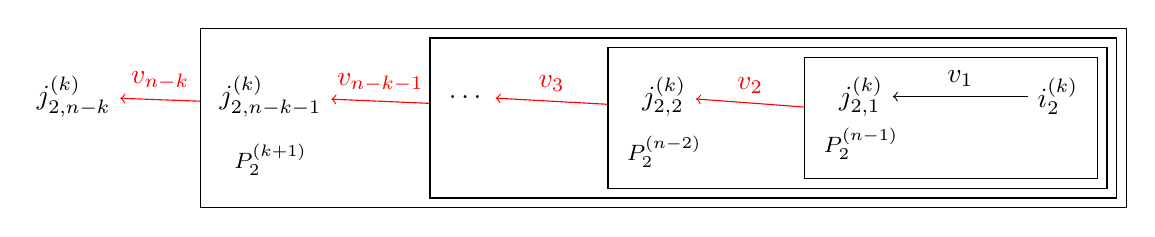
\begin{tikzpicture}
\tikzstyle{box} = [rectangle, minimum width=2cm, minimum height=1cm, text centered, draw=black]
\draw (0,0) node (A) {$j^{(k)}_{2,n-k}$} +(2.5,0) node (B) {$j^{(k)}_{2,n-k-1}$}+(2.5,-.8) node (P1) {\footnotesize$P_2^{(k+1)}$} +(5,0) node (B1) {$\dots$} +(7.5,0) node (C) {$j^{(k)}_{2,2}$} +(7.5,-.7) node (P3) {\footnotesize$P_2^{(n-2)}$}+(10,0) node (D) {$j^{(k)}_{2,1}$}  +(12.5,0) node (E) {$i^{(k)}_2$} +(10,-.6) node (P4) {\footnotesize$P_2^{(n-1)}$}; 
\node (Q1) [draw=black,fit={(D) (E) (P4)}]{};
\node (Q2) [draw=black,fit={(Q1) (C) (P3)}]{};
\node (Q2b)[draw=black,fit={(Q2) (B1) }]{};

\node (Q3)[draw=black,fit={(Q2b) (B) (P1)}]{};
\draw[<-] (D)--(E) node[pos=.5,above] {$v_1$};
\draw[->,red] (Q1)--(C) node[pos=.5,above] {$v_2$};
\draw[->,red] (Q2)--(B1) node[pos=.5,above] {$v_3$};
\draw[->,red] (Q2b)--(B) node[pos=.5,above] {$v_{n-k-1}$};

\draw[->,red] (Q3)--(A) node[pos=.5,above] {$v_{n-k}$};
\end{tikzpicture}
\\

\noindent
where the $2$-arrows are coloured red. As the number of strong successor closed subsets of this $2$-quiver coincides with the number of successor closed subsets of the coefficient quiver, for clearness reasons, we will mostly work with the coefficient quiver instead.

The next step is to define the $2$-quivers of $P^{(k)}_3$ whence the remaining $2$-quivers can be obtained recursively. First we choose the basis of $\Ext(P_2^{(1)},P_2)$ given by the linear maps
$$\{i_2^{(n-1)}\xlongrightarrow{v_n}j_{2,i}\mid i=n-1,\ldots,1\}.$$
This basis gives rise to the following $2$-quiver of $P_3^{(k)}$ where we drop the indices of the vertices in abuse of notation.
\\

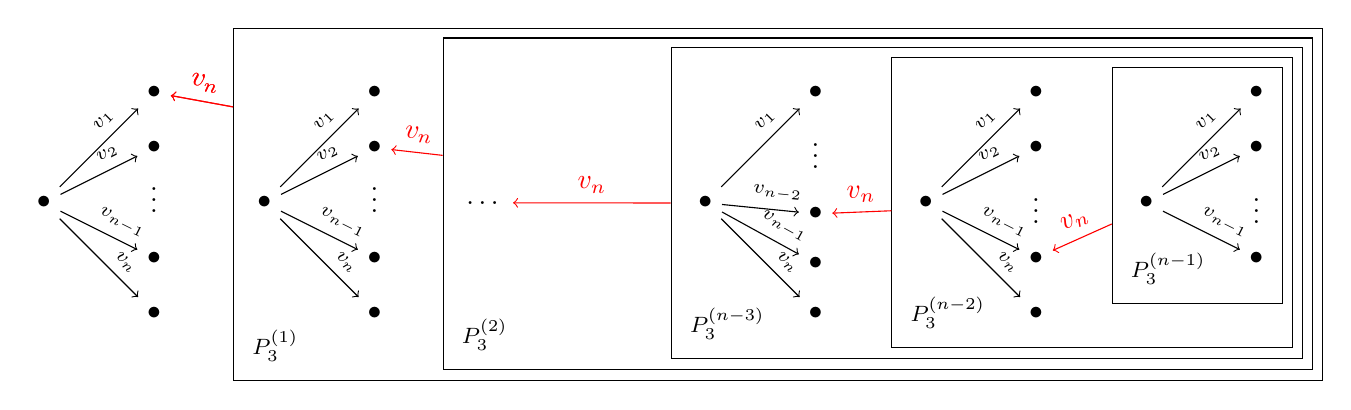
\begin{tikzpicture}[scale=1.4]
\draw (0,0) node (I1) {$\bullet$} +(1,1) node (J11) {$\bullet$} +(1,.5) node (J12) {$\bullet$} +(1,0.1) node (D1) { $\vdots$}+(1,-.5) node (J1N1) {$\bullet$} +(1,-1) node (J1N) {$\bullet$} ; 
\draw[->] (I1)--(J11) node[pos=.7,above,sloped]{\scriptsize$v_1$};
\draw[->] (I1)--(J12) node[pos=.7,above,sloped]{\scriptsize$v_2$};
\draw[->] (I1)--(J1N1) node[pos=.7,above,sloped]{\scriptsize$v_{n-1}$};
\draw[->] (I1)--(J1N) node[pos=.7,above,sloped]{\scriptsize$v_{n}$};

\draw (2,0) node (I2) {$\bullet$} +(1,1) node (J21) {$\bullet$} +(1,.5) node (J22) {$\bullet$}+(1,0.1) node (D2) { $\vdots$} +(1,-.5) node (J2N1) {$\bullet$} +(1,-1) node (J2N) {$\bullet$} +(0.1,-1.3) node (P1) {\footnotesize$P_3^{(1)}$} ; 
\draw[->] (I2)--(J21) node[pos=.7,above,sloped]{\scriptsize$v_1$};
\draw[->] (I2)--(J22) node[pos=.7,above,sloped]{\scriptsize$v_2$};
\draw[->] (I2)--(J2N1) node[pos=.7,above,sloped]{\scriptsize$v_{n-1}$};
\draw[->] (I2)--(J2N) node[pos=.7,above,sloped]{\scriptsize$v_{n}$};

\draw (4,0) node (DOTS) {$\dots$}+(0,-1.2) node (P2b) {\footnotesize$P_3^{(2)}$};

\draw (6,0) node (I3) {$\bullet$} +(1,1) node (J31) {$\bullet$}   +(1,.5) node (D31) { $\vdots$} +(1,-.1) node (J3N2) {$\bullet$} +(1,-.55) node (J3N1) { $\bullet$} +(1,-1) node (J3N) {$\bullet$} +(0.2,-1.1) node (P3) {\footnotesize$P_3^{(n-3)}$} ; 
\draw[->] (I3)--(J31) node[pos=.7,above,sloped]{\scriptsize$v_1$};
\draw[->] (I3)--(J3N2) node[pos=.7,above,sloped]{\scriptsize$v_{n-2}$};
\draw[->] (I3)--(J3N1) node[pos=.7,above,sloped]{\scriptsize$v_{n-1}$};
\draw[->] (I3)--(J3N) node[pos=.7,above,sloped]{\scriptsize$v_{n}$};

\draw (8,0) node (I4) {$\bullet$} +(1,1) node (J41) {$\bullet$} +(1,.5) node (J42) {$\bullet$} +(1,0) node (D4) { $\vdots$} +(1,-.5) node (J4N1) {$\bullet$} +(1,-1) node (J4N) {$\bullet$} +(0.2,-1) node (P4) {\footnotesize$P_3^{(n-2)}$}; 
\draw[->] (I4)--(J41) node[pos=.7,above,sloped]{\scriptsize$v_1$};
\draw[->] (I4)--(J42) node[pos=.7,above,sloped]{\scriptsize$v_2$};
\draw[->] (I4)--(J4N1) node[pos=.7,above,sloped]{\scriptsize$v_{n-1}$};
\draw[->] (I4)--(J4N) node[pos=.7,above,sloped]{\scriptsize$v_{n}$};

\draw (10,0) node (I5) {$\bullet$} +(1,1) node (J51) {$\bullet$} +(1,.5) node (J52) {$\bullet$} +(1,0) node (D5) { $\vdots$} +(1,-.5) node (J5N1) {$\bullet$} +(0.2,-.6) node (P5) {\footnotesize$P_3^{(n-1)}$}   ; 
\draw[->] (I5)--(J51) node[pos=.7,above,sloped]{\scriptsize $v_1$};
\draw[->] (I5)--(J52) node[pos=.7,above,sloped]{\scriptsize $v_2$};
\draw[->] (I5)--(J5N1) node[pos=.7,above,sloped]{\scriptsize $v_{n-1}$};
%\tikzstyle{every node}=[circle,fill=white!10]
\node (Q2) [draw=black,fit={(P5) (I5) (J51) (J52) (J5N1)}]{};
%\node (R2) [draw=black,fit={(I4) (J4N1)}, sloped]{};
\draw[->,red] (Q2)--(J4N1) node[pos=.5,above,sloped]{$v_{n}$};
\node (Q3) [draw=black,fit={(P4) (Q2) (I4) (J41) (J42) (J4N1) (J4N)}]{};
\draw[->,red] (Q3)--(J3N2)  node[pos=.5,above,sloped] {$v_{n}$};
\node (Q4) [draw=black,fit={(P3) (Q3) (I3) (J31) (J3N1) (J3N2) (J3N)}]{};
\draw[->,red] (Q4)--(DOTS)  node[pos=.5,above] {$v_{n}$};
\node (Q4b) [draw=black,fit={(P2b) (Q4) (DOTS)}]{};

\node (Q5) [draw=black,fit={(P1) (Q4b) (I2) (J21) (J22) (J2N1) (J2N)}]{};
\draw[->,red] (Q5)--(J11)  node[pos=.5,above,sloped,sloped] {$v_{n}$};
\draw[->,red] (Q4b)--(J22)  node[pos=.5,above,sloped] {$v_{n}$};
\draw[->,red] (Q5)--(J11)  node[pos=.5,above,sloped] {$v_{n}$};

\end{tikzpicture}
\\

We have $\dim \Hom(P_m,\tau P_m^{(k)})=\dim\Ext(P_m^{(k)},P_m)=n-k$. If a basis of $\Ext(P_m^{(k)},P_m)$ is compatible with a lift to the universal covering, Lemma \ref{AR} gives a one-to-one correspondence between basis elements of $\Ext(P_m^{(k)},P_m)$ and $\Hom(P_{m-1},\tau P_m^{(k)})$. Let us consider the case $m=3$. The coefficient quiver of $\tau P_3^{(k)}$ is given by
\[\xymatrix@R10pt@C20pt{&&i_{1}\ar_{v_1}[lld]\\ j &&\vdots\\&&i_{k}\ar_{v_{k}}[llu]}.\]
The image of the homomorphism of the corresponding exact sequence induced by the basis element $i_2^{(n-1)}\xrightarrow{v_n} j_{2,l}$ is the quotient quiver $j\xlongleftarrow{v_l} i_l$. Thus in this case the $2$-arrow connects the $2$-quiver of $P_3^{(k)}$ to the image of the corresponding homomorphism $P_2\to P_1^{(k)}$ which is of dimension $(1,1)$. In the above illustration, we forgo to insert the corresponding rectangles and just connected the $2$-arrows to the sinks of the corresponding subquivers. It can be seen that this is no restriction from the combinatorial point of view. 

Now we can recursively the $2$-quivers of $P_m^{(k)}$ for $m\geq 4$ and $k=n-1,\ldots,0$ when repeating this procedure. For $m\geq 4$, the truncated preprojective $\tau P_m^{(k)}$ can uniquely be found as a quotient of $P_m$.
Recall that we have $\udim P_m^{(k)}=\udim P_{m-1}^{(1)}+(n-k-1)\udim P_{m-1}$. Moreover, we have 
\[\dim \Hom(P_{m-1},\tau P_m^{(1)})=\dim\Ext(P_m^{(1)},P_{m-1})=n-1.\]

As before we get a one-to-one correspondence between basis elements when passing to the universal covering quiver. More precisely, we can take the BGP-reflected basis of the basis of $\Ext(P_2^{(1)},P_2)$ from above.

Let us assume that we already constructed the $2$-quiver of $P_{m+1}^{(k)}$. The $2$-quiver of $P^{(k-1)}_{m+1}$ is given by glueing the $2$-quiver of $P_{m+1}^{(k)}$ to the one of $P_{m}$
\\

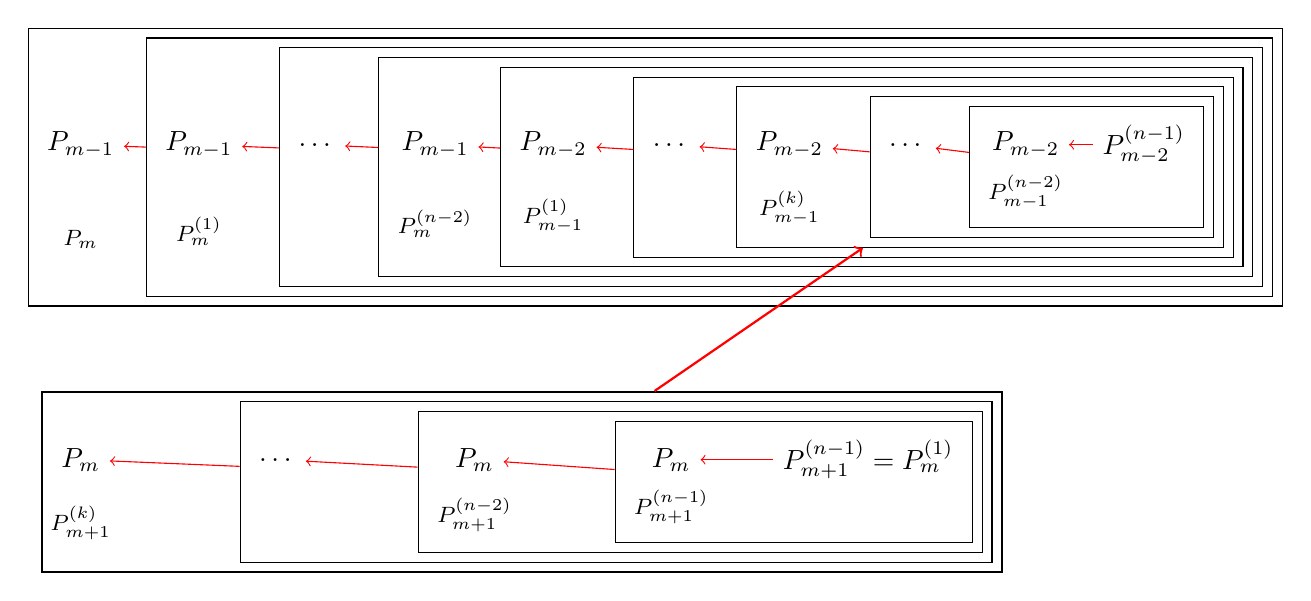
\begin{tikzpicture}
\draw (0,4) node (A1) {$P_{m-1}$}+(0,-1.2) node (PM) {\footnotesize$P_{m}$} +(1.5,0) node (B1) {$P_{m-1}$}+(1.5,-1.1) node (P11) {\footnotesize$P_{m}^{(1)}$} +(3,0) node (B11) {$\dots$} +(4.5,0) node (D1) {$P_{m-1}$}  +(6,0) node (E1) {$P_{m-2}$} +(4.5,-1) node (P41) {\footnotesize$P_{m}^{(n-2)}$}+(6,-.9) node (P51) {\footnotesize$P_{m-1}^{(1)}$}+(7.5,0) node (A1b) {$\dots$} +(9,0) node (B1b) {$P_{m-2}$}+(9,-.8) node (P11b) {\footnotesize$P_{m-1}^{(k)}$} +(10.5,0) node (B11b) {$\dots$} +(12,0) node (D1b) {$P_{m-2}$} +(12,-.6) node (P41b) {\footnotesize$P_{m-1}^{(n-2)}$} +(13.5,0) node (E1b) {$P^{(n-1)}_{m-2}$} ; 
\node (Q11) [draw=black,fit={(D1b) (E1b) (P41b)}]{};
\node (Q21) [draw=black,fit={(Q11) (B11b)}]{};
\node (Q31)[draw=black,fit={(Q21) (B1b) (P11b)}]{};
\node (Q41)[draw=black,fit={(Q31) (A1b)}]{};
\node (Q51)[draw=black,fit={(Q41) (E1)}]{};
\node (Q61)[draw=black,fit={(Q51) (P41) (D1)}]{};
\node (Q71)[draw=black,fit={(Q61) (B11)}]{};
\node (Q81)[draw=black,fit={(Q71) (P11) (B1)}]{};
\node (Q91)[draw=black,fit={(Q81) (A1)}]{};
\draw[<-,red] (D1b)--(E1b) node[pos=.5,above] {};
\draw[->,red] (Q11)--(B11b) node[pos=.5,above] {$$};
\draw[->,red] (Q21)--(B1b) node[pos=.5,above] {$$};
\draw[->,red] (Q31)--(A1b) node[pos=.5,above] {$$};
\draw[->,red] (Q41)--(E1) node[pos=.5,above] {$$};
\draw[->,red] (Q51)--(D1) node[pos=.5,above] {$$};
\draw[->,red] (Q61)--(B11) node[pos=.5,above] {$$};
\draw[->,red] (Q71)--(B1) node[pos=.5,above] {$$};
\draw[->,red] (Q81)--(A1) node[pos=.5,above] {$$};

\draw (0,0) node (B) {$P_{m}$}+(0,-.8) node (P1) {\footnotesize$P_{m+1}^{(k)}$} +(2.5,0) node (B1) {$\dots$} +(5,0) node (C) {$P_{m}$} +(5,-.7) node (P3) {\footnotesize$P_{m+1}^{(n-2)}$}+(7.5,0) node (D) {$P_{m}$}  +(10,0) node (E) {$P_{m+1}^{(n-1)}=P_{m}^{(1)}$} +(7.5,-.6) node (P4) {\footnotesize$P_{m+1}^{(n-1)}$}; 
\node (Q1) [draw=black,fit={(D) (E) (P4)}]{};
\node (Q2) [draw=black,fit={(Q1) (C) (P3)}]{};
\node (Q2b)[draw=black,fit={(Q2) (B1) }]{};

\draw[<-,red] (D)--(E) node[pos=.5,above] {};
\draw[->,red] (Q1)--(C) node[pos=.5,above] {$$};
\draw[->,red] (Q2)--(B1) node[pos=.5,above] {$$};
\draw[->,red] (Q2b)--(B) node[pos=.5,above] {$$};

\node (PMK) [draw=black, thick,fit={(Q2b) (B)}]{};
\draw[->,red,thick] (PMK)--(Q31);
\end{tikzpicture}
\\

\noindent where the $2$-arrows connects the $2$-quiver of $P_{m+1}^{(k)}$ to its Auslander-Reiten translate $\tau P_{m+1}^{(k)}= P_{m-1}^{(k)}$ in $P_m$. This subquiver can be found at the very right of the $2$-quiver of $P_m$. Note that forgo the colouring of the arrows as it does not play any role from the combinatorial point of view. For $n=3$ the $2$-quiver of $P_3$ is given by:\\

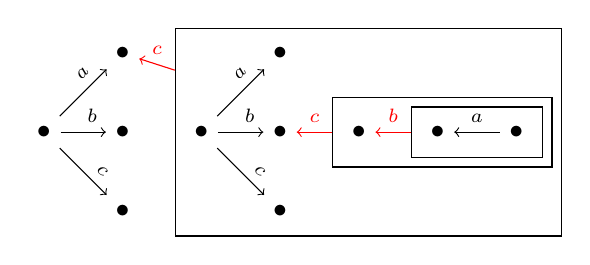
\begin{tikzpicture}[scale=1]
\draw (0,0) node (I1) {$\bullet$} +(1,1) node (J11) {$\bullet$} +(1,0) node (J12) {$\bullet$} +(1,-1) node (J13) {$\bullet$}; 
\draw[->] (I1)--(J11) node[pos=.7,above,sloped]{\scriptsize$a$};
\draw[->] (I1)--(J12) node[pos=.7,above,sloped]{\scriptsize$b$};
\draw[->] (I1)--(J13) node[pos=.7,above,sloped]{\scriptsize$c$};
%\draw[->] (I1)--(J1N) node[pos=.7,above,sloped]{\scriptsize$v_{n}$};

\draw (2,0) node (I2) {$\bullet$} +(1,1) node (J21) {$\bullet$} +(1,0) node (J22) {$\bullet$} +(1,-1) node (J23) {$\bullet$}; 
\draw[->] (I2)--(J21) node[pos=.7,above,sloped]{\scriptsize$a$};
\draw[->] (I2)--(J22) node[pos=.7,above,sloped]{\scriptsize$b$};
\draw[->] (I2)--(J23) node[pos=.7,above,sloped]{\scriptsize$c$};
%\draw[->] (I1)--(J1N) node[pos=.7,above,sloped]{\scriptsize$v_{n}$};
\draw (6,0) node (I3) {$\bullet$} (5,0) node (J31) {$\bullet$} (4,0) node (J33) {$\bullet$}; 
\draw[->] (I3)--(J31) node[pos=.5,above,sloped]{\scriptsize$a$};
%\draw[->] (I3)--(J32) node[pos=.7,above,sloped]{\scriptsize$b$};
%\draw[->] (I3)--(J33) node[pos=.7,above,sloped]{\scriptsize$c$};
%\draw[->] (I1)--(J1N) node[pos=.7,above,sloped]{\scriptsize$v_{n}$};
\node (Q0)[draw=black,fit={(I3) (J31) }]{};
\node (Q1)[draw=black,fit={(Q0) (J33)}]{};
\node (Q2)[draw=black,fit={(Q1) (I2) (J21) (J22) (J23)}]{};

%\node (Q3)[draw=black,fit={(Q2b) (B) (P1)}]{};
\draw[->,red] (Q0)--(J33) node[pos=.5,above] {\scriptsize $b$};
\draw[->,red] (Q1)--(J22) node[pos=.5,above] {\scriptsize $c$};
\draw[->,red] (Q2)--(J11) node[pos=.5,above] {\scriptsize $c$};
\end{tikzpicture}
\\

The one of $P_4$ is given by:\\

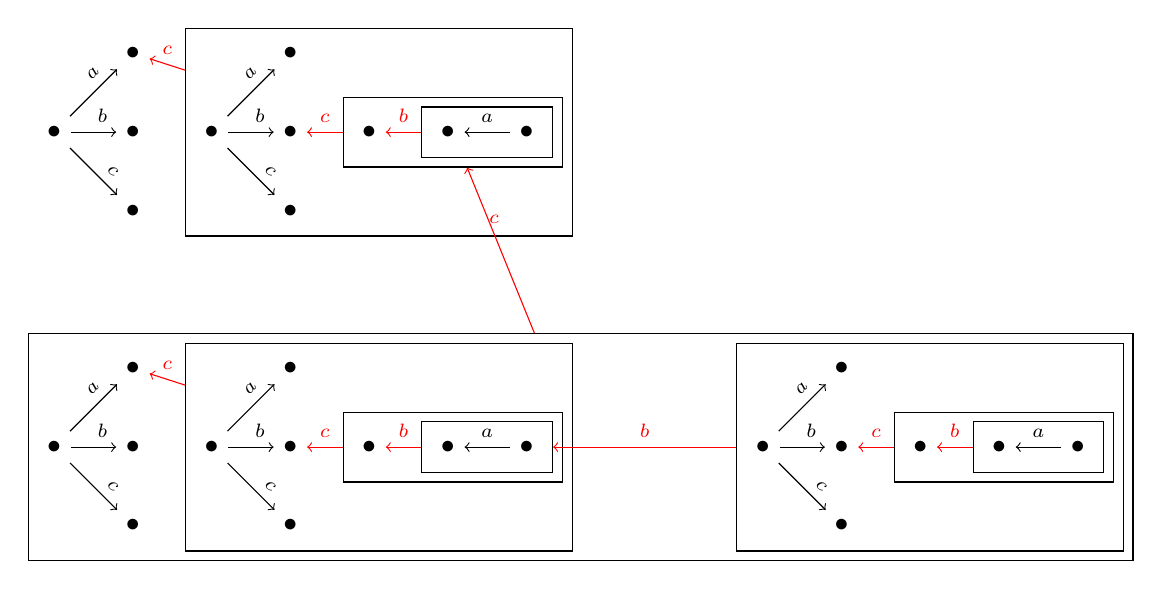
\begin{tikzpicture}[scale=1]
\draw (0,0) node (I1) {$\bullet$} +(1,1) node (J11) {$\bullet$} +(1,0) node (J12) {$\bullet$} +(1,-1) node (J13) {$\bullet$}; 
\draw[->] (I1)--(J11) node[pos=.7,above,sloped]{\scriptsize$a$};
\draw[->] (I1)--(J12) node[pos=.7,above,sloped]{\scriptsize$b$};
\draw[->] (I1)--(J13) node[pos=.7,above,sloped]{\scriptsize$c$};
%\draw[->] (I1)--(J1N) node[pos=.7,above,sloped]{\scriptsize$v_{n}$};

\draw (2,0) node (I2) {$\bullet$} +(1,1) node (J21) {$\bullet$} +(1,0) node (J22) {$\bullet$} +(1,-1) node (J23) {$\bullet$}; 
\draw[->] (I2)--(J21) node[pos=.7,above,sloped]{\scriptsize$a$};
\draw[->] (I2)--(J22) node[pos=.7,above,sloped]{\scriptsize$b$};
\draw[->] (I2)--(J23) node[pos=.7,above,sloped]{\scriptsize$c$};
%\draw[->] (I1)--(J1N) node[pos=.7,above,sloped]{\scriptsize$v_{n}$};
\draw (6,0) node (I3) {$\bullet$} (5,0) node (J31) {$\bullet$} (4,0) node (J33) {$\bullet$}; 
\draw[->] (I3)--(J31) node[pos=.5,above,sloped]{\scriptsize$a$};
%\draw[->] (I3)--(J32) node[pos=.7,above,sloped]{\scriptsize$b$};
%\draw[->] (I3)--(J33) node[pos=.7,above,sloped]{\scriptsize$c$};
%\draw[->] (I1)--(J1N) node[pos=.7,above,sloped]{\scriptsize$v_{n}$};
\node (Q0)[draw=black,fit={(I3) (J31) }]{};
\node (Q1)[draw=black,fit={(Q0) (J33)}]{};
\node (Q2)[draw=black,fit={(Q1) (I2) (J21) (J22) (J23)}]{};

%\node (Q3)[draw=black,fit={(Q2b) (B) (P1)}]{};
\draw[->,red] (Q0)--(J33) node[pos=.5,above] {\scriptsize $b$};
\draw[->,red] (Q1)--(J22) node[pos=.5,above] {\scriptsize $c$};
\draw[->,red] (Q2)--(J11) node[pos=.5,above] {\scriptsize $c$};


\draw (0,-4) node (I1b) {$\bullet$} +(1,1) node (J11b) {$\bullet$} +(1,0) node (J12b) {$\bullet$} +(1,-1) node (J13b) {$\bullet$}; 
\draw[->] (I1b)--(J11b) node[pos=.7,above,sloped]{\scriptsize$a$};
\draw[->] (I1b)--(J12b) node[pos=.7,above,sloped]{\scriptsize$b$};
\draw[->] (I1b)--(J13b) node[pos=.7,above,sloped]{\scriptsize$c$};
%\draw[->] (I1)--(J1N) node[pos=.7,above,sloped]{\scriptsize$v_{n}$};

\draw (2,-4) node (I2b) {$\bullet$} +(1,1) node (J21b) {$\bullet$} +(1,0) node (J22b) {$\bullet$} +(1,-1) node (J23b) {$\bullet$}; 
\draw[->] (I2b)--(J21b) node[pos=.7,above,sloped]{\scriptsize$a$};
\draw[->] (I2b)--(J22b) node[pos=.7,above,sloped]{\scriptsize$b$};
\draw[->] (I2b)--(J23b) node[pos=.7,above,sloped]{\scriptsize$c$};

\draw (6,-4) node (I3b) {$\bullet$} (5,-4) node (J31b) {$\bullet$} (4,-4) node (J33b) {$\bullet$}; 
\draw[->] (I3b)--(J31b) node[pos=.5,above,sloped]{\scriptsize$a$};
\node (Q0b)[draw=black,fit={(I3b) (J31b) }]{};
\node (Q1b)[draw=black,fit={(Q0b) (J33b)}]{};
\node (Q2b)[draw=black,fit={(Q1b) (I2b) (J21b) (J22b) (J23b)}]{};

\draw[->,red] (Q0b)--(J33b) node[pos=.5,above] {\scriptsize $b$};
\draw[->,red] (Q1b)--(J22b) node[pos=.5,above] {\scriptsize $c$};
\draw[->,red] (Q2b)--(J11b) node[pos=.5,above] {\scriptsize $c$};

\draw (9,-4) node (I2c) {$\bullet$} +(1,1) node (J21c) {$\bullet$} +(1,0) node (J22c) {$\bullet$} +(1,-1) node (J23c) {$\bullet$}; 
\draw[->] (I2c)--(J21c) node[pos=.7,above,sloped]{\scriptsize$a$};
\draw[->] (I2c)--(J22c) node[pos=.7,above,sloped]{\scriptsize$b$};
\draw[->] (I2c)--(J23c) node[pos=.7,above,sloped]{\scriptsize$c$};

\draw (13,-4) node (I3c) {$\bullet$} (12,-4) node (J31c) {$\bullet$} (11,-4) node (J33c) {$\bullet$}; 
\draw[->] (I3c)--(J31c) node[pos=.5,above,sloped]{\scriptsize$a$};
\node (Q0c)[draw=black,fit={(I3c) (J31c) }]{};
\node (Q1c)[draw=black,fit={(Q0c) (J33c)}]{};
\node (Q2c)[draw=black,fit={(Q1c) (I2c) (J21c) (J22c) (J23c)}]{};
\node (Q3c)[draw=black,fit={(Q2c) (Q2b) (I1b)}]{};
\draw[->,red] (Q0c)--(J33c) node[pos=.5,above] {\scriptsize $b$};
\draw[->,red] (Q1c)--(J22c) node[pos=.5,above] {\scriptsize $c$};
\draw[->,red] (Q2c)--(Q0b) node[pos=.5,above] {\scriptsize $b$};
\draw[->,red] (Q3c)--(Q1) node[pos=.6,above] {\scriptsize $c$};







\end{tikzpicture}



\begin{theorem}
The Euler characteristic $\chi(\Gr_e(P_m^{(k)}))$ is given by the number of strong successor closed subsets of type $e$ of the $2$-quiver of $P_m^{(k)}$.
\end{theorem}
\begin{proof}
We proceed by induction. The strong successor closed subsets of the $2$-quivers of $P_1$, $P_2$ and $P_2^{(n-1)}$ coincide with the successor closed subsets of the coefficient quivers (\ref{coeff}) which we denote by $\Gamma_M$ for $M\in\{P_1, P_2,P_2^{(n-1)}\}$. Passing to the universal cover, we have $\Gr_e(\tilde M)\in\{\emptyset,\{\pt\}\}$ such that $\Gr_e(\tilde M)=\{\pt\}$ if and only if $e\subset (\Gamma_M)_0$ is successor closed. As the number cells of $\Gr_e(\tilde M)$ and $\Gr_e(M)$ coincide, the claim follows.

Thus assume that the claim is true for $P_m$ (resp. $\tilde P_{m}$) and $P_{m+1}^{(k)}$ (resp. $\tilde P_{m+1}^{(k)}$) and consider the short exact sequence
\[\ses{\tilde P_m}{\tilde P_{m+1}^{(k-1)}}{\tilde P_{m+1}^{(k)}}.\]
Denote the corresponding $2$-quivers by $\Gamma_{P_m}$ and $\Gamma_{P_{m+1}^{(k)}}$ and let $\beta_1\cup\beta_2\subset (\Gamma_{P_m})_0\cup (\Gamma_{P_{m+1}^{(k)}})_0$ be a pair of strong successor closed subsets which gives rise to a pair of non-empty cell by induction hypothesis. Denote by $d(\beta_1+\beta_2)$ the dimension vector corresponding to this subset. By Proposition \ref{fibers} the pair $\beta_1\cup\beta_2$, it does not correspond to a non-empty cell of $\Gr_{d(\beta_1+\beta_2)}(\tilde P_{m+1}^{(k)})$ if and only if $\beta_2=(\Gamma_{P_{m+1}^{(k)}})_0$ and $\beta_1\cap(\Gamma_{\tau\tilde P_{m+1}^{(k)}})_0=\emptyset$. But this is precisely the condition on $\beta_1\cup\beta_2$ to be strong successor closed as $\Gamma_{P_{m+1}^{(k)}}$ is connected to $\Gamma_{\tau\tilde P_{m+1}^{(k)}}$ by a $2$-arrow.

\end{proof}

\begin{thebibliography}{10}
\bibitem{ass}
Assem, I., Simson, D., Skowronski, A.: Elements of the Representation Theory of Associative Algebras. Cambridge University Press, Cambridge 2007.
\bibitem{bb} Bialynicki-Birula, A.: Some theorems on actions of algebraic groups. Annals of Mathematics \textbf{98}, 480-497 (1973).
\bibitem{bgp}
Bernstein, I.~N., Gelfand, I.~M., Ponomarev, V.~A.: Coxeter functors, and Gabriel's theorem. Russian Mathematical Surveys \textbf{28}(2), 17-32 (1973).
\bibitem{brenner-butler} S. Benner, M.~C.~R. Butler, The equivalence of certain functors occuring in the representation theory of artin algebras and species, J. London Math. Soc., 14 (1976), 183-187.
\bibitem{cc}
Caldero, P., Chapoton, F.: Cluster algebras as {H}all algebras of quiver representations.
Commentarii Mathematici Helvetici \textbf{81}(3), 595-616 (2006).
\bibitem{ck}
  P. Caldero, B. Keller: From triangulated categories to cluster algebras II.  Ann. Sci. \'Ecole Norm. Sup. (4) \textbf{39} (2006), no. 6, pp.~983--1009.
\bibitem{cefr} Cerulli Irelli, Esposito, Franzen, Reineke: Topology of Quiver Grassmannians. Preprint 2017.
\bibitem{cr}
Caldero, P., Reineke, M.: On the quiver Grassmannian in the acyclic case.
Journal of Pure and Applied Algebra \textbf{212}(11), 2369-2380 (2008).
\bibitem{cj} Crawley-Boevey, W., Jensen, Bernt Tore: A note on sub-bundles of vector bundles. Glasgow Mathematical Journal \textbf{48}, 459-462 (2006).

\bibitem{gab} Gabriel, P.: The universal cover of a finite-dimensional algebra. Representations of algebras. Lecture Notes in Mathematics {\bf 903}, 68-105 (1981).
\bibitem{hr} Happel, D., Ringel, C.M.: Tilted Algebras. Transactions of the American Mathematical Society {\bf 274}, no.2, 399-443 (1982).
\bibitem{llz} K. Lee, L. Li, A. Zelevinsky: Greedy elements in rank 2 cluster algebras. Selecta Math. \textbf{20} (2014) pp.~57--82.
\bibitem{rin} Ringel, C.M.: Reflection functors for hereditary algebras. Journal of the London Mathematical Society (2) {\bf 21}, no. 3, 465-479 (1980).
%\bibitem{mats} Matsumura, H.: Commutative ring theory. 
\bibitem{rupel} Rupel, D.: Rank Two Non-Commutative Laurent Phenomenon and Pseudo-Positivity, arXiv.

\bibitem{sch} Schofield, A.: General representations of quivers. Proceedings of the London Mathematical Society (3) \textbf{65}(1), 46-64 (1992).
	\bibitem{wei} Weist, T.: Localization of quiver moduli spaces. Representation Theory \textbf{17}(13), 382-425 (2013).
\end{thebibliography}

\end{document}
